%% ****** Start of file apsguide4-2.tex ****** %
%%
%%   This file is part of the APS files in the REVTeX 4.2 distribution.
%%   Version 4.2b of REVTeX, December 2018.
%%
%%   Copyright (c) 2019 The American Physical Society.
%%
%%   See the REVTeX 4.2 README file for restrictions and more information.
%%
\documentclass[twocolumn,secnumarabic,amssymb, nobibnotes, aps, prd]{revtex4-2}
\usepackage{graphicx}
\usepackage{subfigure}
\usepackage{hyperref}
%\usepackage{acrofont}%NOTE: Comment out this line for the release version!
\usepackage{amssymb}
\usepackage{xcolor}

\newcommand{\revtex}{REV\TeX\ }
\newcommand{\classoption}[1]{\texttt{#1}}
\newcommand{\macro}[1]{\texttt{\textbackslash#1}}
\newcommand{\m}[1]{\macro{#1}}
\newcommand{\env}[1]{\texttt{#1}}
\setlength{\textheight}{9.5in}

\hypersetup{
    colorlinks,
    urlcolor={black},
    % linkcolor={blue!80!black},
    linkcolor={black},
    citecolor=black
}

\begin{document}

\title{Classroom learning dynamics using a cellular automata spatiotemporal model comparing peer instruction and traditional instruction}%

\author{Clarence Ioakim T. Sy}%
\affiliation{National Institute of Physics, University of the Philippines Diliman, Quezon City, Philippines}%

\author{Ranzivelle Marianne L. Roxas-Villanueva}%
\affiliation{Institute of Physics, University of the Philippines Los Ba\~{n}os, Laguna, Philippines}%

\author{Johnrob Y. Bantang}%
\email[Corresponding author: ]{jybantang@up.edu.ph}
\affiliation{National Institute of Physics, University of the Philippines Diliman, Quezon City, Philippines}%

\date{June 2025}%

\begin{abstract}
    Peer instruction (PI) has become \textcolor{red}{one of the popular means} of classroom instruction in Physics Education.
    Such instruction method is vastly different from how classes are traditionally handled where the instructor conducts a lecture for the entire duration of the class.
    In this study, we model the \textcolor{red}{learning} within classes of students as a probabilistic cellular automata model 
    and investigate the effects of different factors such as seating arrangements, class size $N$, average learning rate ${\lambda}$, and heterogeneity $\delta{\lambda}$ on the class overall learning efficiency.
    The learning efficiency of the class is measured in terms of the overall class rate \textcolor{red}{using the total learning time $t_{\rm max}$} for the whole class.
    PI mode appears to be more applicable with heterogeneous classes (in-class high learning rate max difference $\delta{\lambda}$).
    As commonly known TI mode is shown to be more advantageous for large $N$ and homogenous class aptitude (low $\delta{\lambda}$).
    % High learning rate of students benefits both TI and PI but in different ways.
    We show that the learning curves of highly heterogeneous classes with TI mode have two stages of learning: a fast initial stage and a slow final stage.
    The slow final state class learning rate is due to the late learners with lower $\lambda$-values and have general shape dependent on other model parameters as well.
    Such curves are absent with PI which consistently shifts depending on the other factors.
    Differing from a previous empirical data for the PI mode, classes perform best when the best in the class are situated within the inner corner.
    The model we used for this study currently ignores the actual non-isotropic seating orientation with which students do not share knowledge readily in all neighboring seating directions.
    Our model simplified the student capabilities to binary values and does not consider the \textcolor{red}{positive} effect of aptitude similarity during peer interactions as described in previous studies.
    We therefore find that PI \textcolor{red}{performs better than, or similar to,} traditional instruction.
    A mix of TI and PI would be the optimal mode of instruction taking advantage of TI for fast learning in the initial stage and the robust learning curve of PI in the later stages of class learning.
    Despite these simplifications, our model is able to provide general insights that are in agreement with previous studies and existing practices.
\end{abstract}

\maketitle
\tableofcontents

\section{Introduction}

%    Literature discussing peer instruction, especially for physics often cites Mazur's work \textit{Peer Instruction: A User's Manual} .
%    In this book, Mazur recounts how he observed a disconnect between students' ability to answer quantitative and conceptual questions in physics.
    Peer instruction (PI)--an increasingly popular method of instruction--attempts to solve a disconnect between students' ability to answer quantitative and conceptual questions, particularly in physics subject matters~\cite{mazur1997peer,mazur1999}.
%    He concluded that this resulted from the students' approach of memorizing problem solving algorithms, even if they might not always apply to a given problem.
	Such disconnect is said to be attributed to the typical approach of memorizing physics problem patterns and applying the same solution patterns regardless of their potential non-applicability.
%    Peer Instruction (PI) as a method of instruction aims to address this issue.
    The PI method forces students to think critically and to engage with peers guided by the learning material as opposed to simply absorbing the information from lectures given by the instructor as in the traditional mode of instruction (TI).
    The method's effectivity has been shown not only in high school physics settings, but also in other disciplines and higher education settings~\cite{johnson2008active,fagen2000factors,fagen2002peer}.

%%%%%%%%%%%%%%%
%%    \subsection{Difference of Peer Instruction from Traditional Instruction}

%    There are many ways to implement PI in the classroom.
%    The method outlined by Mazur~\cite{mazur1997peer} involves the instructor giving a short lecture on a topic, followed by a multiple choice question (MCQ) that the students answer individually.
%    The students then discuss their answers with their peers before answering an MCQ again.
%    Variations can be made depending on the class set up and the instructor.
    
    The PI method as outlined by Mazur and Somers~\cite{mazur1997peer} typically involves an instructor giving a short lecture on the topic, followed by a multiple-choice question (MCQ) that the student answer individually.
    PI emphasizes on the next phases of instruction which involve repeated cycle of students sharing their answers to the MCQ and discussing them with peers, usually until they get the concepts right.
    This part makes the PI method student centric requiring the instructor to intervene with slightly modified steps to adjust to the needs of the class.
    As long as the same learning objectives are tackled, the instructor can choose variations in the method~\cite{smith2009peer}.
    The instructor may often decide on: increasing the multiplicity of the peer sharing and discussion phase; having different kinds of requirements and/or levels of evaluation~\cite{crouch2001peer}; providing different MCQ sets; or giving another short lecture to ensure clarity of concepts involved~\cite{lasry2008peer}.
    Modifications to the PI method have also been reported to minimize some undesired behavioral patterns such as just copying off each other~\cite{smith2009peer}.
    The PI therefore contrasts significantly against the traditional method (TI) with which the instructor simply gives a lecture for the entire duration, typically with minimal peer interactions among the students during class time.
    
%    This is in stark contrast with how traditional instruction (TI) is conducted where the instructor often just gives a lecture for the entire duration of the class.
%    PI is meant to be student centric, meaning that the instructor is expected to make differences to the steps outlined above to adjust to the class's needs.
%    The MCQs can be graded or ungraded~\cite{crouch2001peer}, the instructor can choose to give multiple MCQs and peer discussion opportunities during one class, or the instructor can choose to give a different MCQ after the discussion as long as it still tackles the same learning objective~\cite{smith2009peer}.
%    If only a few students answer the MCQ correctly, the instructor can even give a short lecture to clarify the concept~\cite{lasry2008peer}.

%%%%%%%%%%%%%%%
%%    \subsection{Benefits of PI}
%
%    Despite the de-emphasis on problem-solving in PI lectures, students' quantitative problem-solving skills were not compromised and was even improved compared to traditional instruction in some cases.
%    PI was also shown to significantly decrease the number of students with extremely low scores~\cite{crouch2001peer}.
%    This is consistent with findings of other studies~\cite{lasry2008peer,thacker1994comparing}.
%    Similarly, students' conceptual understanding of the lessons also improved.
%    This holds true for both in-class concept tests and end-of-semester exams~\cite{crouch2001peer}.
    
    Despite the unique approach of de-emphasizing actual problem-solving during the PI lecture phase, quantitative problem-solving skills have been consistently shown to remain uncompromised, and in many cases even improved, relative to TI.
    Several advantages were pointed out in favor of the PI method in relation to the following dimensions: decrease in the number of students with extremely low scores~\cite{crouch2001peer,lasry2008peer,thacker1994comparing}, improved conceptual understanding~\cite{crouch2001peer}, as well as being independent of the background knowledge~\cite{lasry2008peer,tobias1990they}.


%    Smith, et. al~\cite{smith2009peer} modified the PI method to make sure that students were not copying off of each other. After the first MCQ, he did not show the class's answer statistics and used a pair of isomorphic questions for the MCQs before and after the peer discussion section. Isomorphic questions are questions that tackle the same learning objectives but have different "cover stories".
%    They also found that even in groups whose members were not able to answer the first MCQ, students were able to get the correct answer for the second MCQ.
%    This contradicts the transmissionist view of PI where students only learn from other students who already know the lesson.
%    The study provides evidence that PI can be viewed as constructivist where students learn on their own through discussion and not simply from hearing the correct answer.

%    In addition to those mentioned above Lasry, et. al.~\cite{lasry2008peer} showed that PI is not necessarily dependent on background knowledge. They found that students in under PI performed as well as or better than those under TI despite the former having less background knowledge.
%    They also found the PI greatly reduced the number of students who dropped the course.
%    An older paper by Tobias~\cite{tobias1990they} suggests that this could be because of the shift of focus of PI from competition and skill performance to cooperative learning and conceptual understanding.

    The dynamics of the learning process involved during PI is complex resulting from the forced interaction during the peer discussion stage.
    Existing mathematical models for this are either predictive such as with the case of the artificial neural network (ANN) models~\cite{roxas2010seating} or lack the spatial aspect of the process such as utilizing differential equations~\cite{pritchard2008mathematical,nitta2019mathematical}.
    Somewhat in between these is a generalized Ising model by Bordogna and Albano~\cite{bordogna2001theoretical,bordogna2003simulation} that considers three sources of information for the student to learn from: teacher instruction, peer interaction, and bibliographic materials (books, lecture notes, etc.).
    Their model shows that students learn more when they engage discussions with their peers than those who only listen to lectures.
    They also show that group structure affects student learning, and that low aptitude students may learn at the expense of high aptitude peers---a transmissionist view of PI.
    A survey of many other mathematical techniques are found in the work of \citet{nitta2019mathematical}.
    We are yet to find mathematical models for learning that compares PI with TI.
    
    % The work of \citet{nitta2019mathematical} surveys known models for learning under PI mode.
    % The model of \citet{pritchard2008mathematical} for example uses the quantities that correspond to the levels that each student knows about the given knowledge domain.
    % Representing the portions of known as $K$ and unknown as $U$, we have $K+U=1$.
    % Pritchard et al.~\cite{pritchard2008mathematical} uses a set of differential equations that is dependent on the probability of students learning to stick (memory model, Equation~\ref{eq:memory model}) and the ability for students to associate new learnings from old knowledge via logistic differential equation (connectedness model, Equation~\ref{eq:connectedness model}.)
% %%
%     They proceed using a memory model such that the portion of unknown over time follows
%     \begin{equation}
%         \label{eq:memory model}
%         \frac{dU(t)}{dt} = -m U(t)
%     \end{equation}
% %%
%     and with the assumption of a connectedness model gives
%     \begin{equation}
%         \label{eq:connectedness model}
%         \frac{dU(t)}{dt} = -c U(t)K(t),
%     \end{equation}
% %%
%     where knowledge is taken to grow at a uniform rate, as in the Tutoring model:
%     \begin{eqnarray}
%         K(t) &=& {\alpha}t + K_0 \label{eq:tutoring model} \\
%         U(t) + K(T) &=& 1
%     \end{eqnarray}
% %%
%     Where $U(t)$ and $K(t)$ are the unknown and known knowledge domains respectively.
%     The parameters $\alpha_m$, $\alpha_c$, and $\alpha_{tu}$ are the corresponding rates for the memory model, connectedness model, and tutoring model ....

%     In deriving their own model of PI, Nitta arrived at analytic equations similar to the Hake gain to evaluate the effectiveness of PI for a concept test question (Equation~\ref{eq: PIE}) and Pritchard's connectedness model (Equation~\ref{eq:connectedness model}) to model students' learning after each MCQ (Equation~\ref{eq: nitta model}).

%     \begin{equation}
%         \label{eq: PIE}
%         \eta(q) \equiv \frac{\rho_2(q;c)-\rho_1(q;c)}{1-\rho_1(q;c)}
%     \end{equation}

%     \begin{equation}
%         \label{eq: nitta model}
%         \rho_2 = \rho_1 +\rho_1(1-\rho_1)
%     \end{equation}

%     Comparing their equations to data, they concluded that these metrics and equations roughly agree with the data and could give us insights on the learning dynamics of the classroom.

    Actual assessment results by \citet{roxas2010seating} is used to train their ANN to predict expected second assessment scores of students depending on seating arrangements.
% The artificial neural network (ANN) model by \citet{roxas2010seating} used actual assessment results to train a neural network to map student interactions in PI classrooms. 
    Using this neural network, they were also able to characterize \textcolor{red}{students' learning} and investigate the effects of group homogeneity. 
    Their study revealed that an optimal seating arrangement exists for students under PI methods based on their final aptitude.
    In their paper, the measure of each students' improvement was calculated via the Hake gain~\cite{hake1998} as 
    %%
    $g \equiv (S_2 - S_1) / (1 - S_1)$
    %%
    where $S_1$ and $S_2$ are scores for respectively first and second assessment.
    They also used the output/input ratio ($O/I = S_2/S_1$) to gauge student improvement.
    Class improvement is the average of any of the scores.
    % However, it should be noted that $O/I$-values tend to be biased towards low-scoring students.

    The results of their study show that the outer corner seating arrangement (SA) performed the best using both the Hake gain and the $O/I$, followed by inner corner, then random, then center.
    The seating arrangements are illustrated in Fig.~\ref{fig:PI-SAs}.
    In simulated classrooms (ANN system), each with $64$ students and $10$ classrooms in total, they found that homogenous classrooms with low aptitudes have significantly higher $O/I$-values \textcolor{red}{under PI}.
    This means that low aptitude students benefit the most from being grouped together.
    %%
    \begin{figure}[htb]
        \centering
        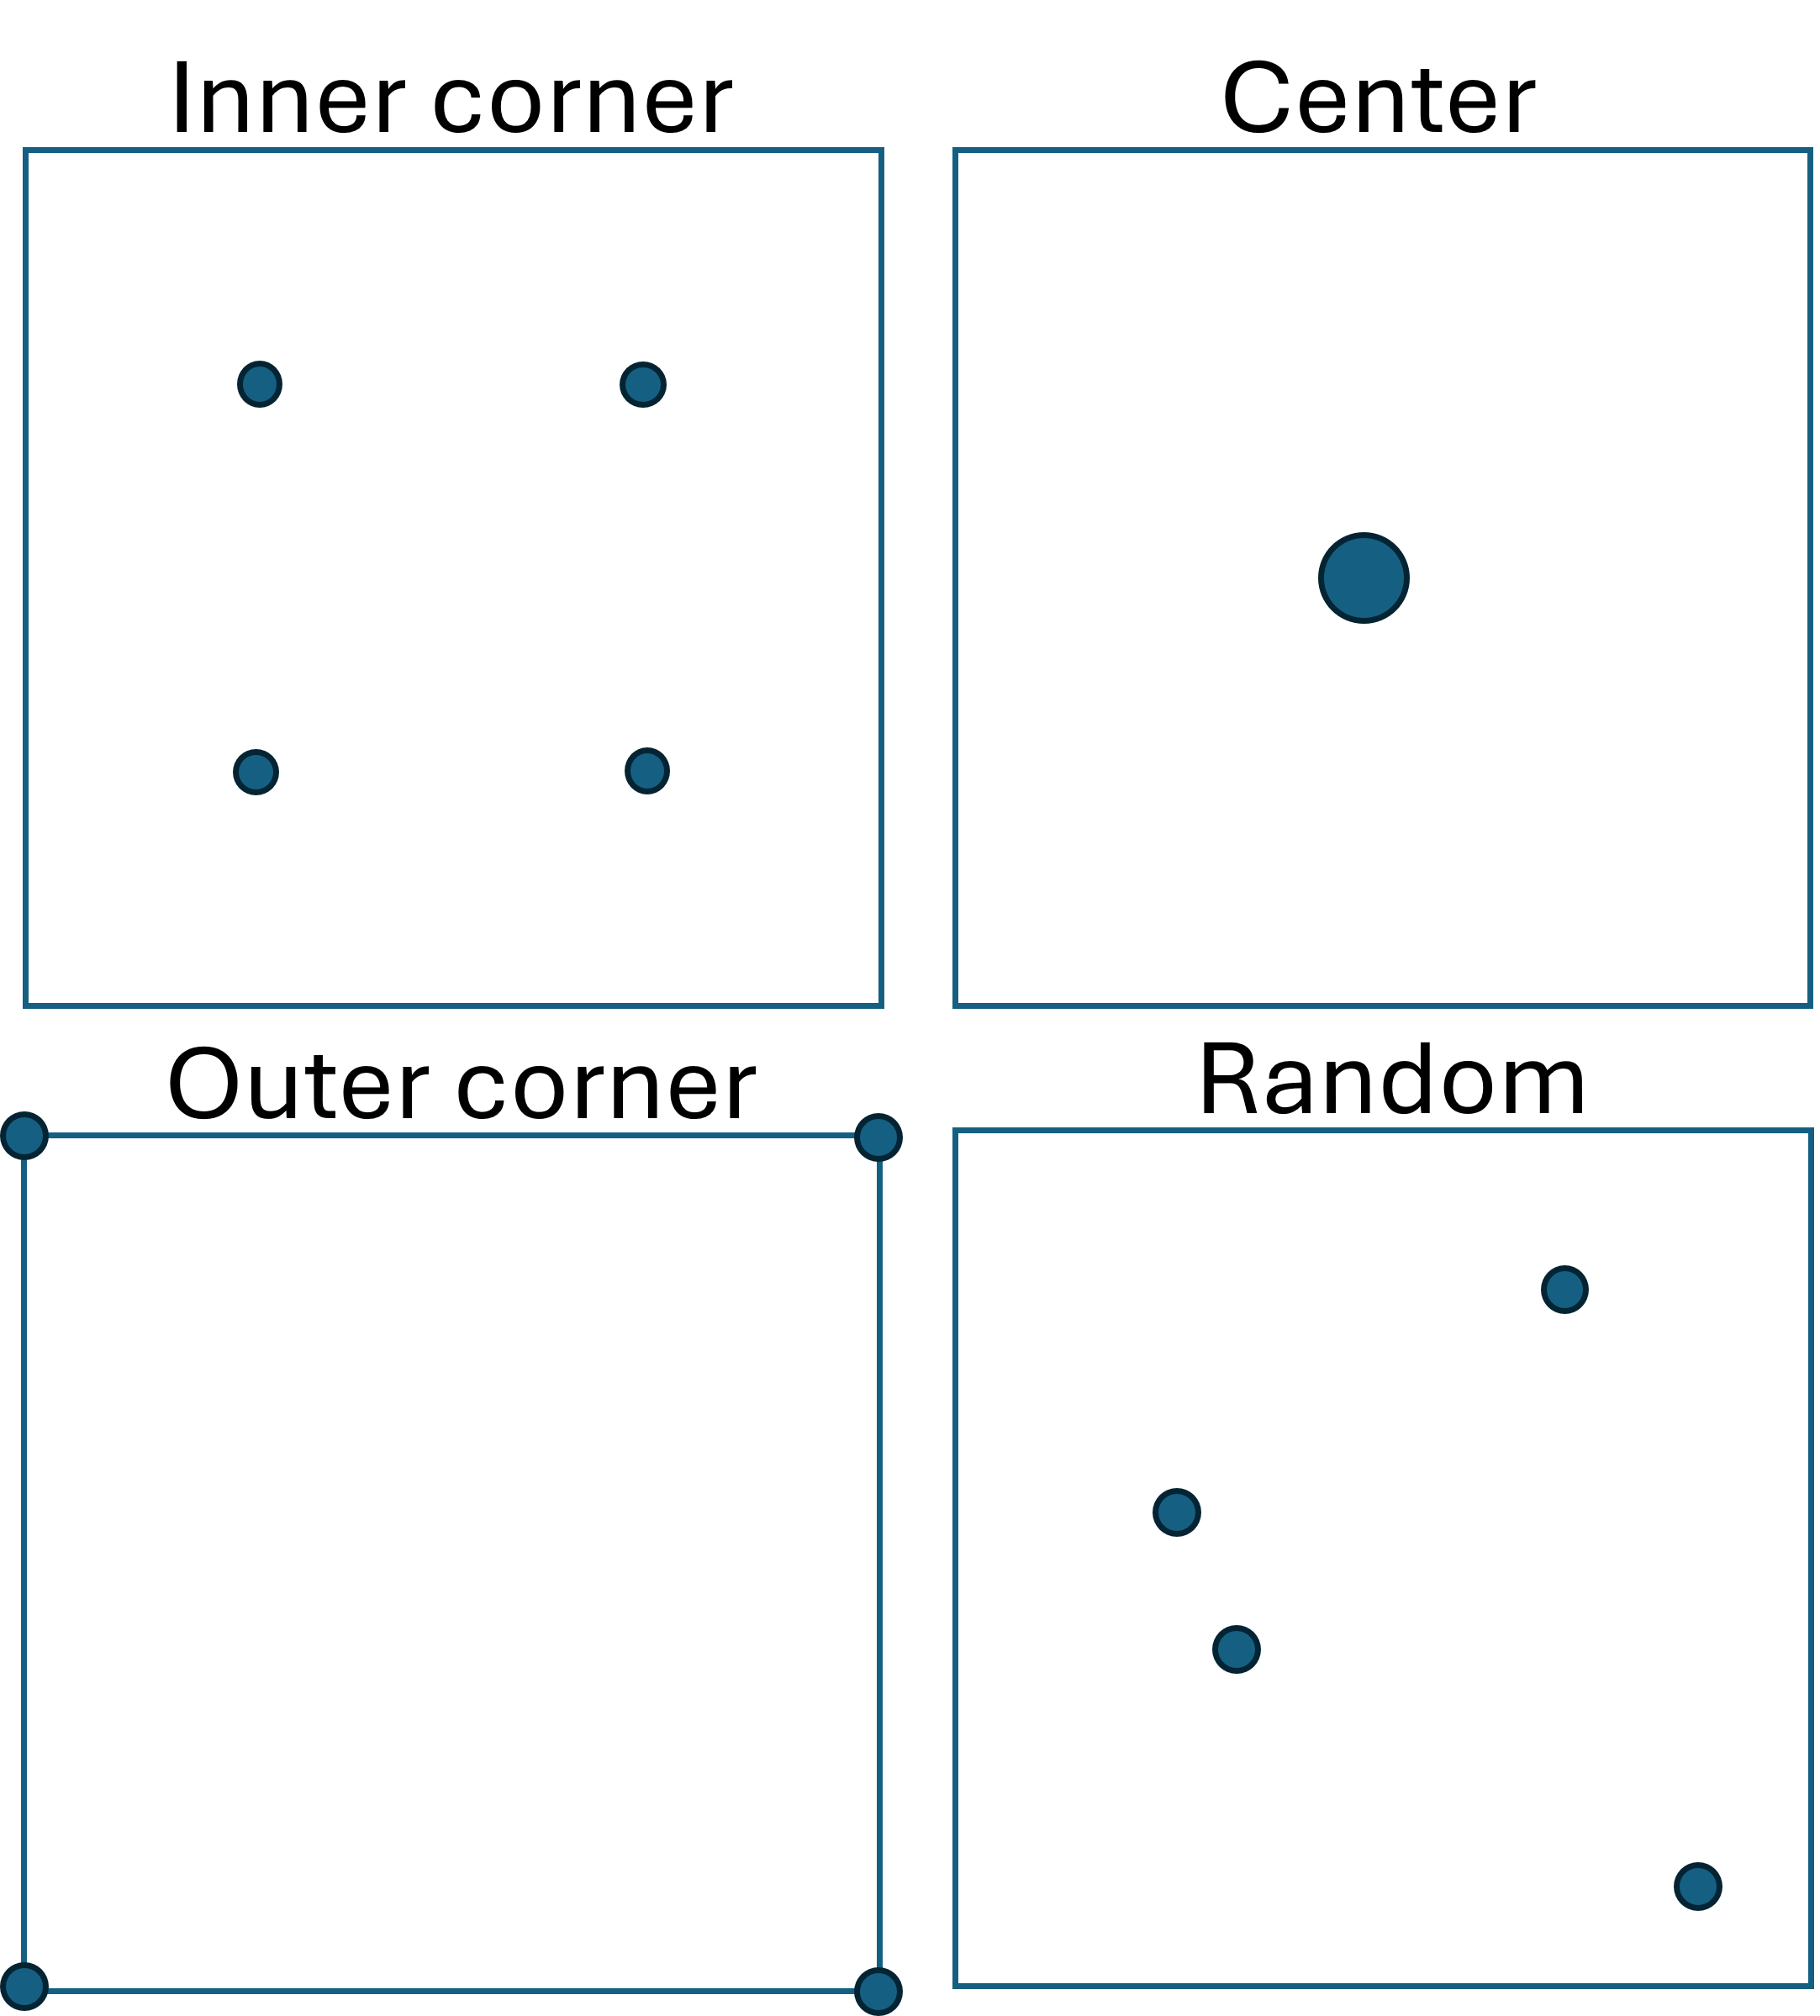
\includegraphics[width=0.30\textwidth]{figures/PI SAs.png}
        \caption{%%
        Seating arrangements considered for PI.
        Dots represent position of high aptitude students.
        The position of other students \textcolor{red}{is} typically arranged in rectangular pattern across the room (here square for brevity).
        The random case is just one of the many possible arrangements.
        }
        \label{fig:PI-SAs}
    \end{figure}

    Hake gain predicts the following expression for the expected score $S_2$ during the assessment after the first such that when done iteratively, every next assessment $S_2$ is dependent on the first assessment score $S_1$ as follows.
    %%
    \begin{equation}
        S_2 = S_1 + g\cdot(1-S_1)
        \label{eq:nitta_model}
    \end{equation}
    %%
    where $g$ may be a function of $S_1$.
    \citet{nitta2019mathematical} presented a model of PI learning that relates the probabilities that the students answers the MCQ correctly (effectively, post- and pre-test).
    Such probabilities would then imply that the Nitta Model predicts that the gain is dependent on the previous score such that:
    %%
    \begin{equation}
        g = g(S_1) = S_1.
        \label{eq:nitta_gain}
    \end{equation}
    %%
    \textcolor{red}{
        Other models provide Hake gain expressions (e.g. \citet{pritchard2008mathematical} \ref{eq:pritchard_connectedness_gain}) resulting to more complex formulation for the function $g(S_1)$.
        This model considers other factors that may affect the learning process.
        $K_{ext}$ is knoweldge that students have that did were not part of the assessment and $\alpha_{memory}$ and $\alpha_{connected}$ are probabilities of learning and information being retained respectively.
        %%
        \begin{equation}
            g = 1 - \exp{ \lbrace - \lbrack \alpha_{memory} (1-\beta) + \alpha_{connected} \beta K_{ext} \rbrack  t \rbrace}
            \label{eq:pritchard_connectedness_gain}
        \end{equation}
    }

    Despite the diversity of the models that we found, current models of PI lack some aspects that we would like to incorporate together like seating arrangements, students' learning rate, and aptitude heterogeneity with which the introduction of PI from TI are typically founded on.
    
\section{Cellular Automata Method}

    We use a probabilistic cellular automata (pCA) model~\cite{SelfSPP} (also known as stochastic cellular automata~\cite{arciaga2009experimental,Batac2009,louis2018probabilistic,Fernandez2018}) to study the spatio-temporal dynamics of learning for a more direct implementation of any instructional mode.
    For this pCA model, each cell in the automaton represents a student arranged in such a way each student is adjacent to (a CA {\it neighbor} of) four others resulting to the usual rectangular lattice configuration.
    For the rectangular lattice, we assign the unique position $(i,j)$ to each student such that $i,j\in[1,L]$ and the classroom size is $N=L^2$.
    The students at the edges and corners have less number of neighbors as in the real situations.

    Each student at every lattice position $(i,j)$ is then assigned a learning rate
    $\lambda_{i,j} \in \mathcal{R}$ 
    as a quantification of how fast they learn as an individual with
    $0{\leq}\lambda_{i,j}{\leq}1$
    (or a probability to learn from any other neighbor).
    This parameter is directly related to the learning aptitude of the students such that we consider the fast learners to have {\it high aptitude score} ($\lambda{\gg}0$).
    We also introduce the state $s_{i,j}$ representing degree of knowledge of the student such that in this work we use
    $s_{i,j}\in\lbrace{0,1}\rbrace$
    as a two-level distinction between {\it learned} (or high-scoring student, $s_{i,j}=1$) and {\it unlearned} (low-scoring, $0$).
    The choice of two-level state should not prevent the possibility of having more levels as long as they can be quantitatively discriminated.

    For each time step, $t\;{\leftarrow}\;(t+1)$, each student's state $s_{i,j}$ is updated depending on the mode of instruction described in the following.
    We use an algorithm (see Fig.~\ref{fig:pCA-flowchart}) general enough to contain various modes of instructions.
    The mode of instructions defines how $P_{i,j}$ is obtained.
    %%%
    \begin{figure}[htb]
        \centering
        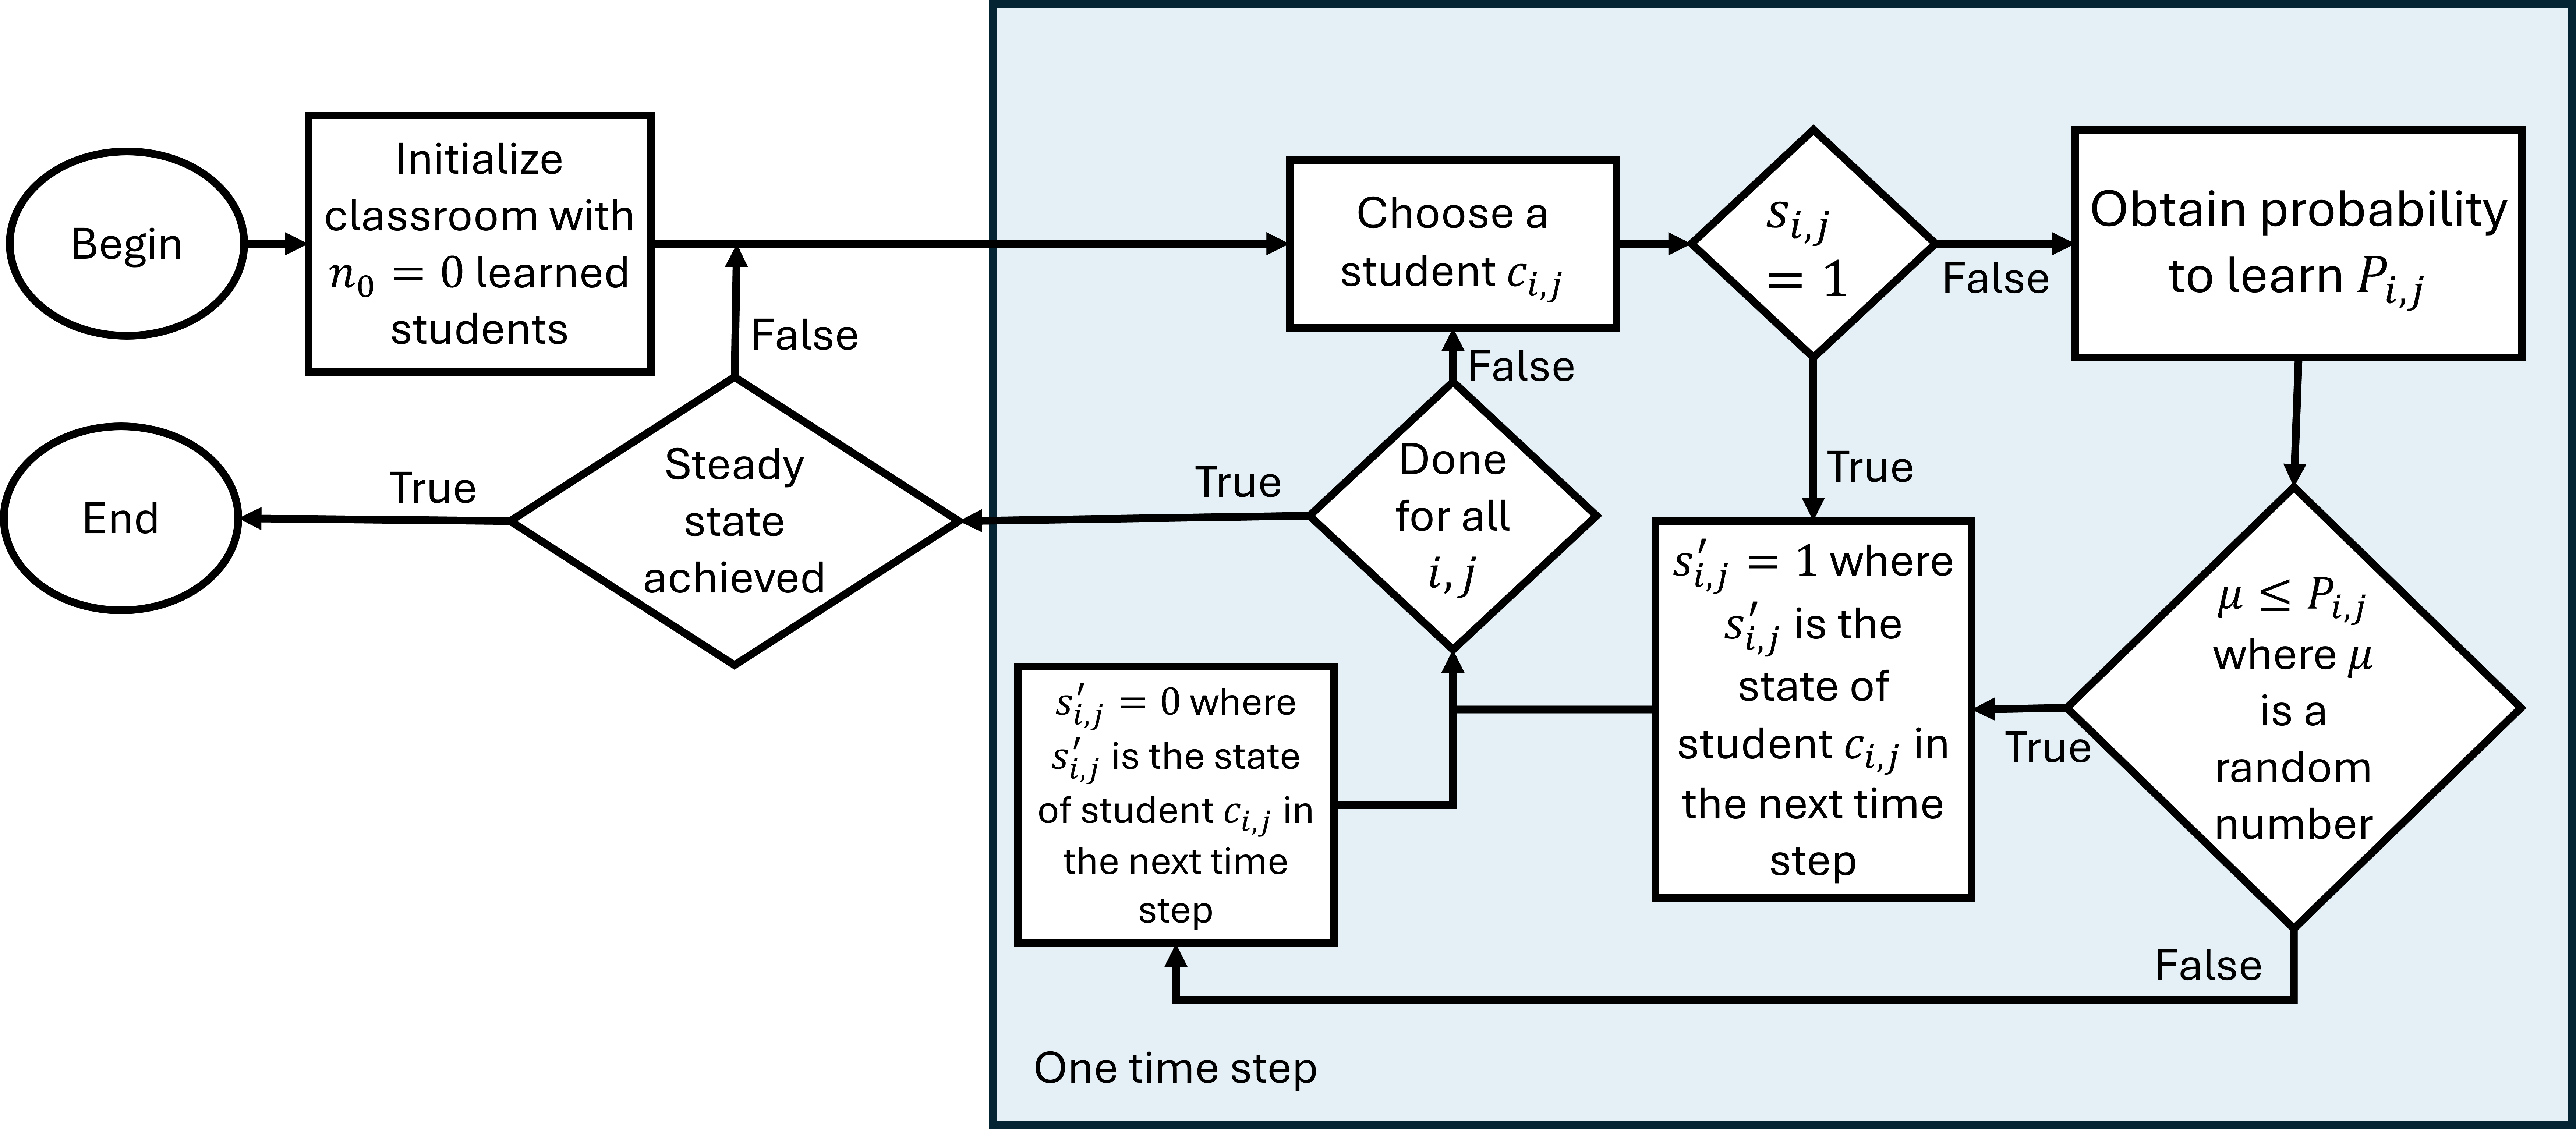
\includegraphics[width=0.45\textwidth]{figures/2DBPCA Flowchart.png}
        \caption{%%
            Flowchart for the pCA algorithm.
            The PI and TI differ on how the probability $P_{i,j}$ is obtained as described in the text.
        }\label{fig:pCA-flowchart}
    \end{figure}

    %%%%TRADITIONAL INSTRUCTION%%%%%

    For traditional instruction (TI) mode, the probability of a student to learn in each time step ($P_{i,j}$) is
    %%
    \begin{equation}
        P_{i,j} = \lambda_{i,j}\;\rho_{\delta i,\delta j}
    \end{equation}
    %%
    with $\rho_{\delta i,\delta j}\in[0,1]$ as the potential dependence of \textcolor{red}{learning} efficiency on the relative position $(\delta i, \delta j)$ of the source of learning (inspiration, input, interaction, discussion, etc.) with respect to the student position $(i,j)$~\cite{dong2021influence}.
    The relative position of the student may matter since instructors in TI mode, for example, may be dependent on the row $i$ since usually students near the front ($i=1$) tend to be more attentive and engaged in discussions than those in the last row ($i=L$).
    To futher simplify for TI, we fix $\rho_{\delta i,\delta j}=\rho_{0}$ as the probability of the students to learn from the teacher directly as if during an efficient plenary (or broadcast) lecture throughout the class such that we simply have $P_{i,j} = \lambda_{i,j}\rho_0$.

    %%%%%PEER INSTRUCTION%%%%%%

    Different from TI, the Peer Instruction mode involves some learning during interaction with peers.
    Such interaction happens with the nearest neighbor unless specific instructions say different.
    We consider the simple case such that the probability $P_{i,j}$ is dependent also on the states of the nearest neighbor.
    In this case, we have a compounded probabilities resulting to
    % the probability of a student to learn in each time step for PI is additionally dependent on the student's neighbors and their states. The probability of a student to learn in each time step ($P_{i,j}$) is given by:
    %%
    \begin{equation} 
        \label{eq:BPCA PI learning probability}
            P_{i,j} = 1 - \prod_{\forall \delta i, \delta j}{\lbrack
                1-(\lambda_{i,j}\;\rho_{\delta i, \delta j})(s_{i+\delta i, j+\delta j})}
            \rbrack
    \end{equation}
    %%
    where we now have dependence on the state
    $s_{i',j'}$ ($i'=i+\delta i$ and $j'=j+\delta j$) factored in every probability of learning transmission.
    We also consider the simplified case such that $\rho_{\delta i, \delta j} = 0$ 
    for $|\delta i| > 1$ and $|\delta j| > 1$ and $\rho_{\delta i,\delta j}=\rho_0$ (fixed, isotropic).
    This assumption translates to the class maintaining their seat arrangement in a lattice pattern and that peer instruction can be modelled as essentially nearest-neighbor interaction only (we use Moore neighborhood)~\cite{kari2005catheory, zaitsev2017generalized,louis2018probabilistic}, although higher degree neighborhood interactions are possible~\cite{dong2021influence}.

    The model allows incorporation of class heterogeneity due to variation in the learning rates of the students such as by specifying the distribution function for random assignment of $\lambda$-values.
    A variation about a fixed rate $\lambda_0=0.5$ is chosen for this work such that $\lambda_{i,j}=\lambda_0 \pm \delta\!\lambda$ (two-level heterogeneity).
    The value of $\delta\!\lambda$ acts as the parameter that determines the degree of class heterogeneity as it is tuned from $0$ to less than $0.5$ (we are limited by the probability range ${0}<\lambda_{i,j}<{1}$).
    We have to remove the case $\delta\lambda=0.5$ that makes the model unrealistic (having $\lambda=0$).
%%
    %%%%MODEL PARAMETERS%%%%
%%
%     The values of the model input parameters we considered for the class size $N=L^2$, the positional learning coefficient $\rho_0$, and the learning rate heterogeneity $\delta\lambda$ are as follows:
% %%
%     \begin{itemize}
%     \item $L=\lbrace32,48,64,96,128\rbrace$
%     \item $\rho_0=\lbrace0.1, 0.2, 0.3,\dots, 0.8, 0.9, 1.0\rbrace$
%     \item $\delta\lambda=\lbrace0.0, 0.1, 0.2, 0.3, 0.4\rbrace$
%     \end{itemize}



    %! Further investigation:
    %! When comparing learning rate of TI vs PI, TI is lower - wrong based on observation. The way we obtained learning rate m does not capture the two-stage learning process of TI. Will omit on this paper because I don't know how to fix that.
    %! TLDR: obtaining m leads to some kind of sampling error. Not the first time.

    % The class's average learning rate $m$ was calculated by taking the fraction of learned students as a function of time then fitting a power law ($y=ax^m$) to a fraction of the data using the Levenberg-Marquardt algorithm.
    % We chose to fit the power law only to the first half or quarter of the data for peer instruction and traditional instruction respectively so that we obtain the class learning rate before the finite size effect become significant.

\section{Results and Discussion}
    
    All TI simulations start with no learned students, while PI simulations start with four ($4$) learned students.
    Class performance is measured as the speed of learning.
    Differences in the dynamical development over time of the class overall state is also observed.
    Here, we use the time $t_{\rm max}$ (in arbitrary units, a.u.) it takes for the entire class to reach a steady state.
    This steady state is considered reached during the numerical experiments when no new student is recorded to have transitioned from {\it unlearned} ($s=0$) to {\it learned} ($s=1$).
    This consideration prevents us from having unnecessary waiting time for the student of very low learning rate $\lambda$ to have $s=1$.
    The average quantities and standard errors are based on twenty($20$) independent randomized runs.

    \subsection{Dynamical Difference between TI and PI}
        Figure~\ref{fig:comparison size} shows the different monotonic increase in the fraction of students in the learned state starting with an unlearned class (all students in {\it unlearned} state).
        For the PI mode, we set to have four($4$) learned students to initiate the spread.
        These are the first four students with the highest aptitude in the class.
        The effect of increasing size of the class $N$ for PI is to delay the time it takes for the class to speed up learning.
        As for the TI mode, an increase in class size $N$ does not affect the dynamics of the learning process.
        This is expected since each student independently and simultaneously learns from the teacher.

        Figure~\ref{fig:comparison ρ₀} shows the same for varying the positional learning factor $\rho_0$.
        A high value for $\rho_0$ increase the initial number of learned students in TI mode.
        In TI mode, the rate of learning is also affected by $\rho_0$ such that the higher the value, the faster the class learns.
        However, in PI mode, the shape of the learning curve remains the same for different values of $\rho_0$, only adding a time delay to when the learning starts to speed up.
        The effect of varying $\rho_0$ is nonlinear for both models.
        The difference between $\rho_0=0.1$ and $\rho_0=0.5$ is greater than that of $\rho_0=0.5$ and $\rho_0=0.9$.
        
        Figure~\ref{fig:comparison δλ} shows the effect of varying the learning rate heterogeneity $\delta\lambda$.
        The effect of $\delta\lambda$ is similar to that of $\rho_0$ in its effects on the dynamics of the learning process and the rate at which students learn throughout the simulation.
        As with $\rho_0$, the effect of $\delta\lambda$ is nonlinear --- the difference between $\delta\lambda=0.4$ and $\delta\lambda=0.2$ is greater than that of $\delta\lambda=0.2$ and $\delta\lambda=0.0$.

    % For TI, varying the different model parameters yield different dynamics.
    %     As shown in Figure~\ref{fig:comparison size}, the progression of the fraction of learned students was not affected with increasing class size $N$.
    %     The time to learn $t_{\rm max}$, however, increased with class size $N$.
    %     This is expected as TI is set up such that the students can all learn at the same time from the teacher --- so the dynamics are independent of class size $N$.
    %     Positional learning factor $\rho_0$ changes the initial number of learned students and the rate at which students learn throughout the simulation (Figure~\ref{fig:comparison ρ₀}).
        
        % Upon initial inspection of Figure~\ref{fig:comparison δλ} for the effects of learning rate heterogeneous, we see that it has a similar effect to that of positional learning factor $\rho_0$ without changing the initial number of learned students.
        % However, we notice that the effect is on the rate of which students learn is not linear.
        % The difference between $\delta\lambda=0.4$ and $\delta\lambda=0.2$ is greater than that of $\delta\lambda=0.2$ and $\delta\lambda=0.0$.
        % This is consistent with the nonlinear effect of $\rho_0$ on the learning rate.
        
        Upon further inspection, we notice that TI classes with high learning rate heterogeneity $\delta\lambda$ have a two-stage learning process.
        The first stage is characterized by a sharp increase in the number of learned students caused by the majority of fast students ($\lambda=\lambda_0 + \delta\lambda$) learning in the first few time steps.
        The second stage is characterized by a much slower increase in the number of learned students caused by waiting for the slower students ($\lambda=\lambda_0 - \delta\lambda$) to learn.
        
        An example case where this phenomenon is observable is shown in Figure~\ref{fig:class_evolution}(a).
        In this case, we see at $t=2$ that majority of the students that are learned are fast students and at $t=13$ the slower students have started to learn, but the rate of learning has slowed down significantly.
        Despite the promising-looking start to this simulation, it will spend up to $t=161$ waiting for all the students to learn.

        % When we vary class size $N$, as shown in Figure~\ref{fig:comparison size}, we see that in TI remains constant with only time to learn $t_{\rm max}$ increasing with class size $N$.
        % For PI, increasing class size $N$ adds a time delay to when the learning starts to speed up. Despite the added time delay, the shape of the learning curve remains the same.
        % The increase in time to learn $t_{\rm max}$ is also less pronounced in PI compared to TI.

        \begin{figure}[htbp!]
            \centering
            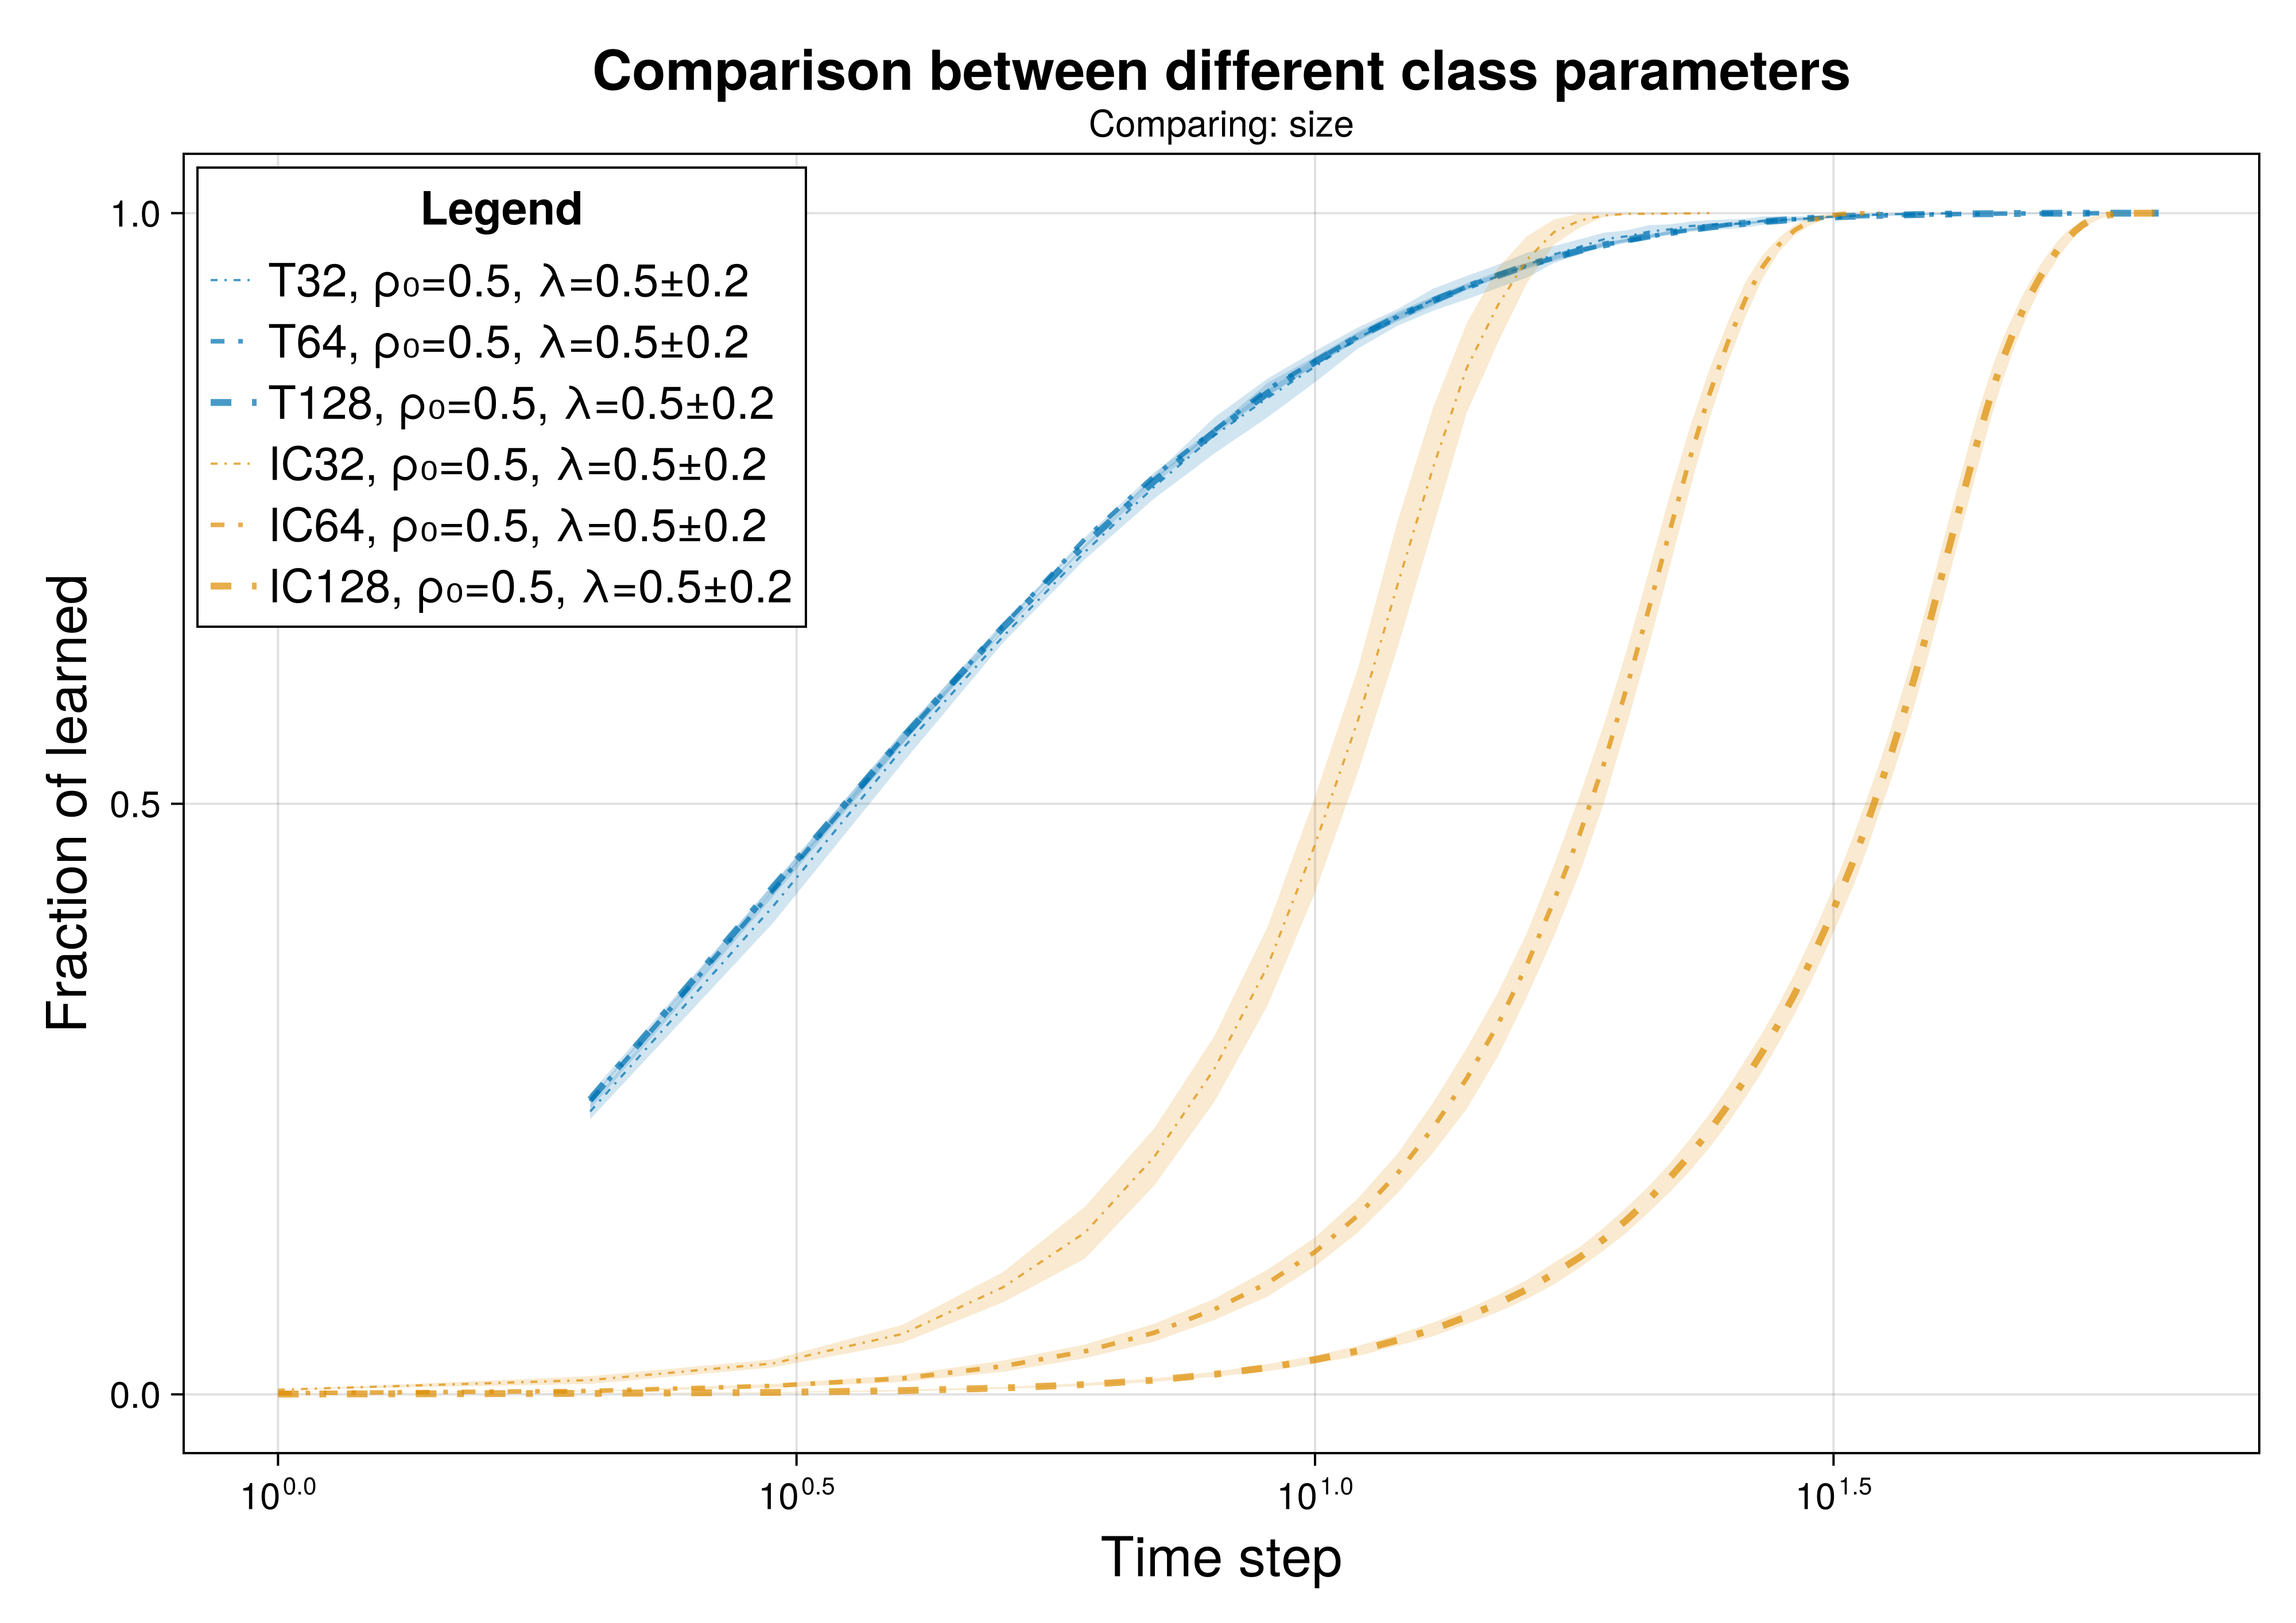
\includegraphics[width=0.45\textwidth]{figures/2D-BPCAIH-analysis/comparison plots/size.png}
            \caption{Comparison of time to learn $t_{\rm max}$ and fraction of learned students for different class sizes $N$.
            Each method of instruction corresponds to a different color --- blue for traditional, orange for inner corner.
            Different class sizes correspond to different line widths where bigger classroom sizes are represented by thicker lines.
            Other parameters are fixed at $\rho_0=0.5$ and $\delta\lambda=0.2$.
            The bands around each line show the standard deviation of the data over $20$ trials.
            Higher fraction of learned students indicate better learning.}
            \label{fig:comparison size}
        \end{figure}

        % Varying positional learning factor $\rho_0$, shown in Figure~\ref{fig:comparison ρ₀}, varies the shape of the learning curve for TI, especially for lower values of positional learning factor $\rho_0$.
        % For traditional instruction, changes in $\rho_0$ affects the number of students that learn in the second time step and the rate of which students learn throughout the class.
        % For peer instruction, the shape of the learning curve remains the same for different values of $\rho_0$, only adding a time delay to when the learning starts to speed up --- similar to the effects of class size $N$.
        % Additionally, the effect of varying positional learning factor $\rho_0$ is nonlinear for both models. Those with extremely low values of $\rho_0$, like those of $\rho_0=0.1$, perform much worse with learning curves being further from $\rho_0=0.5$ than $\rho_0=0.9$ is with $\rho_0=0.5$.

        \begin{figure}[htbp!]
            \centering
            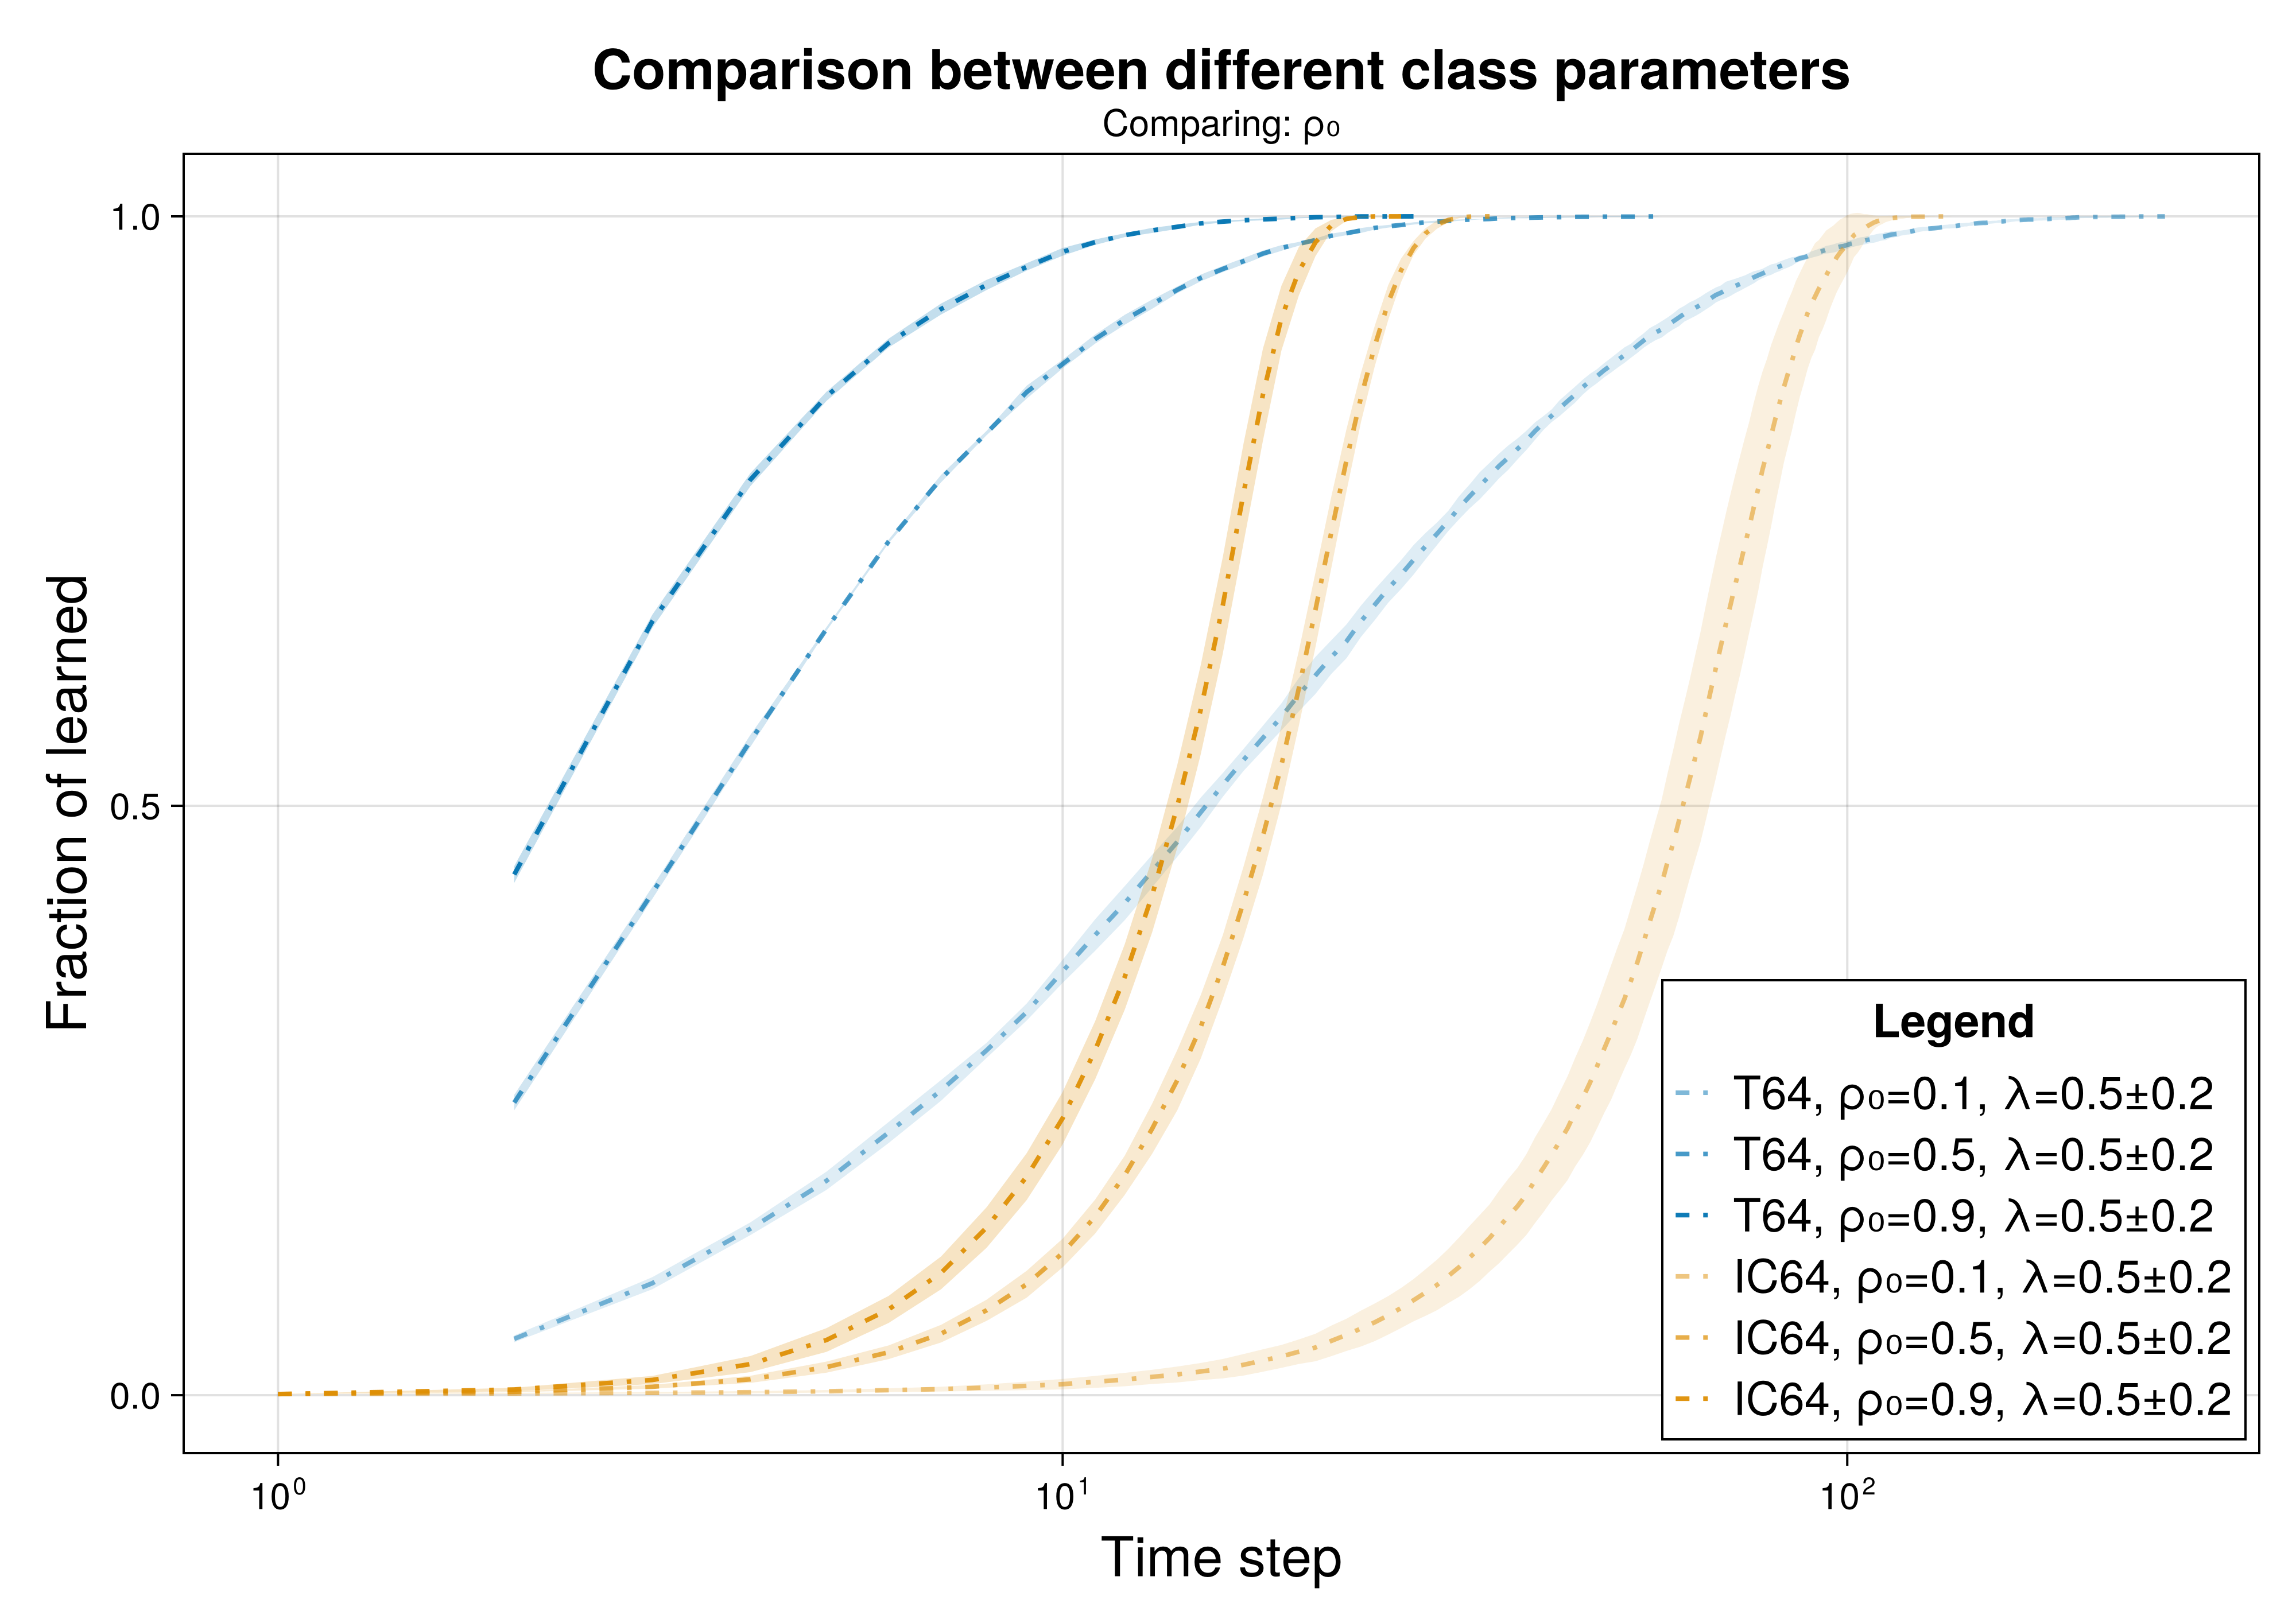
\includegraphics[width=0.45\textwidth]{figures/2D-BPCAIH-analysis/comparison plots/ρ₀.png}
            \caption{Comparison of time to learn $t_{\rm max}$ and fraction of learned students for different values of positional learning factor $\rho_0$.
            Each method of instruction corresponds to a different color --- blue for traditional, orange for inner corner.
            Different $\rho_0$ values correspond to different line transparencies where darker lines represent higher $\rho_0$ values.
            Other parameters are fixed at $N=64$ and $\delta\lambda=0.2$.
            The bands around each line show the standard deviation of the data over $20$ trials.
            Higher fraction of learned students indicate better learning.}
            \label{fig:comparison ρ₀}
        \end{figure}

        % Figure~\ref{fig:comparison δλ} shows that an increase in heterogeneity $\delta\lambda$ changes how fast the slope of the learning curve changes for TI without changing the initial number of learned students.
        % For PI, only very high values of heterogeneity $\delta\lambda$ noticeably affect the learning curve.
        % As with the positional learning factor $\rho_0$, the effect of varying heterogeneity $\delta\lambda$ is similar to that of class size $N$ --- only adding a time delay to when the learning starts to speed up.

        \begin{figure}[htbp!]
            \centering
            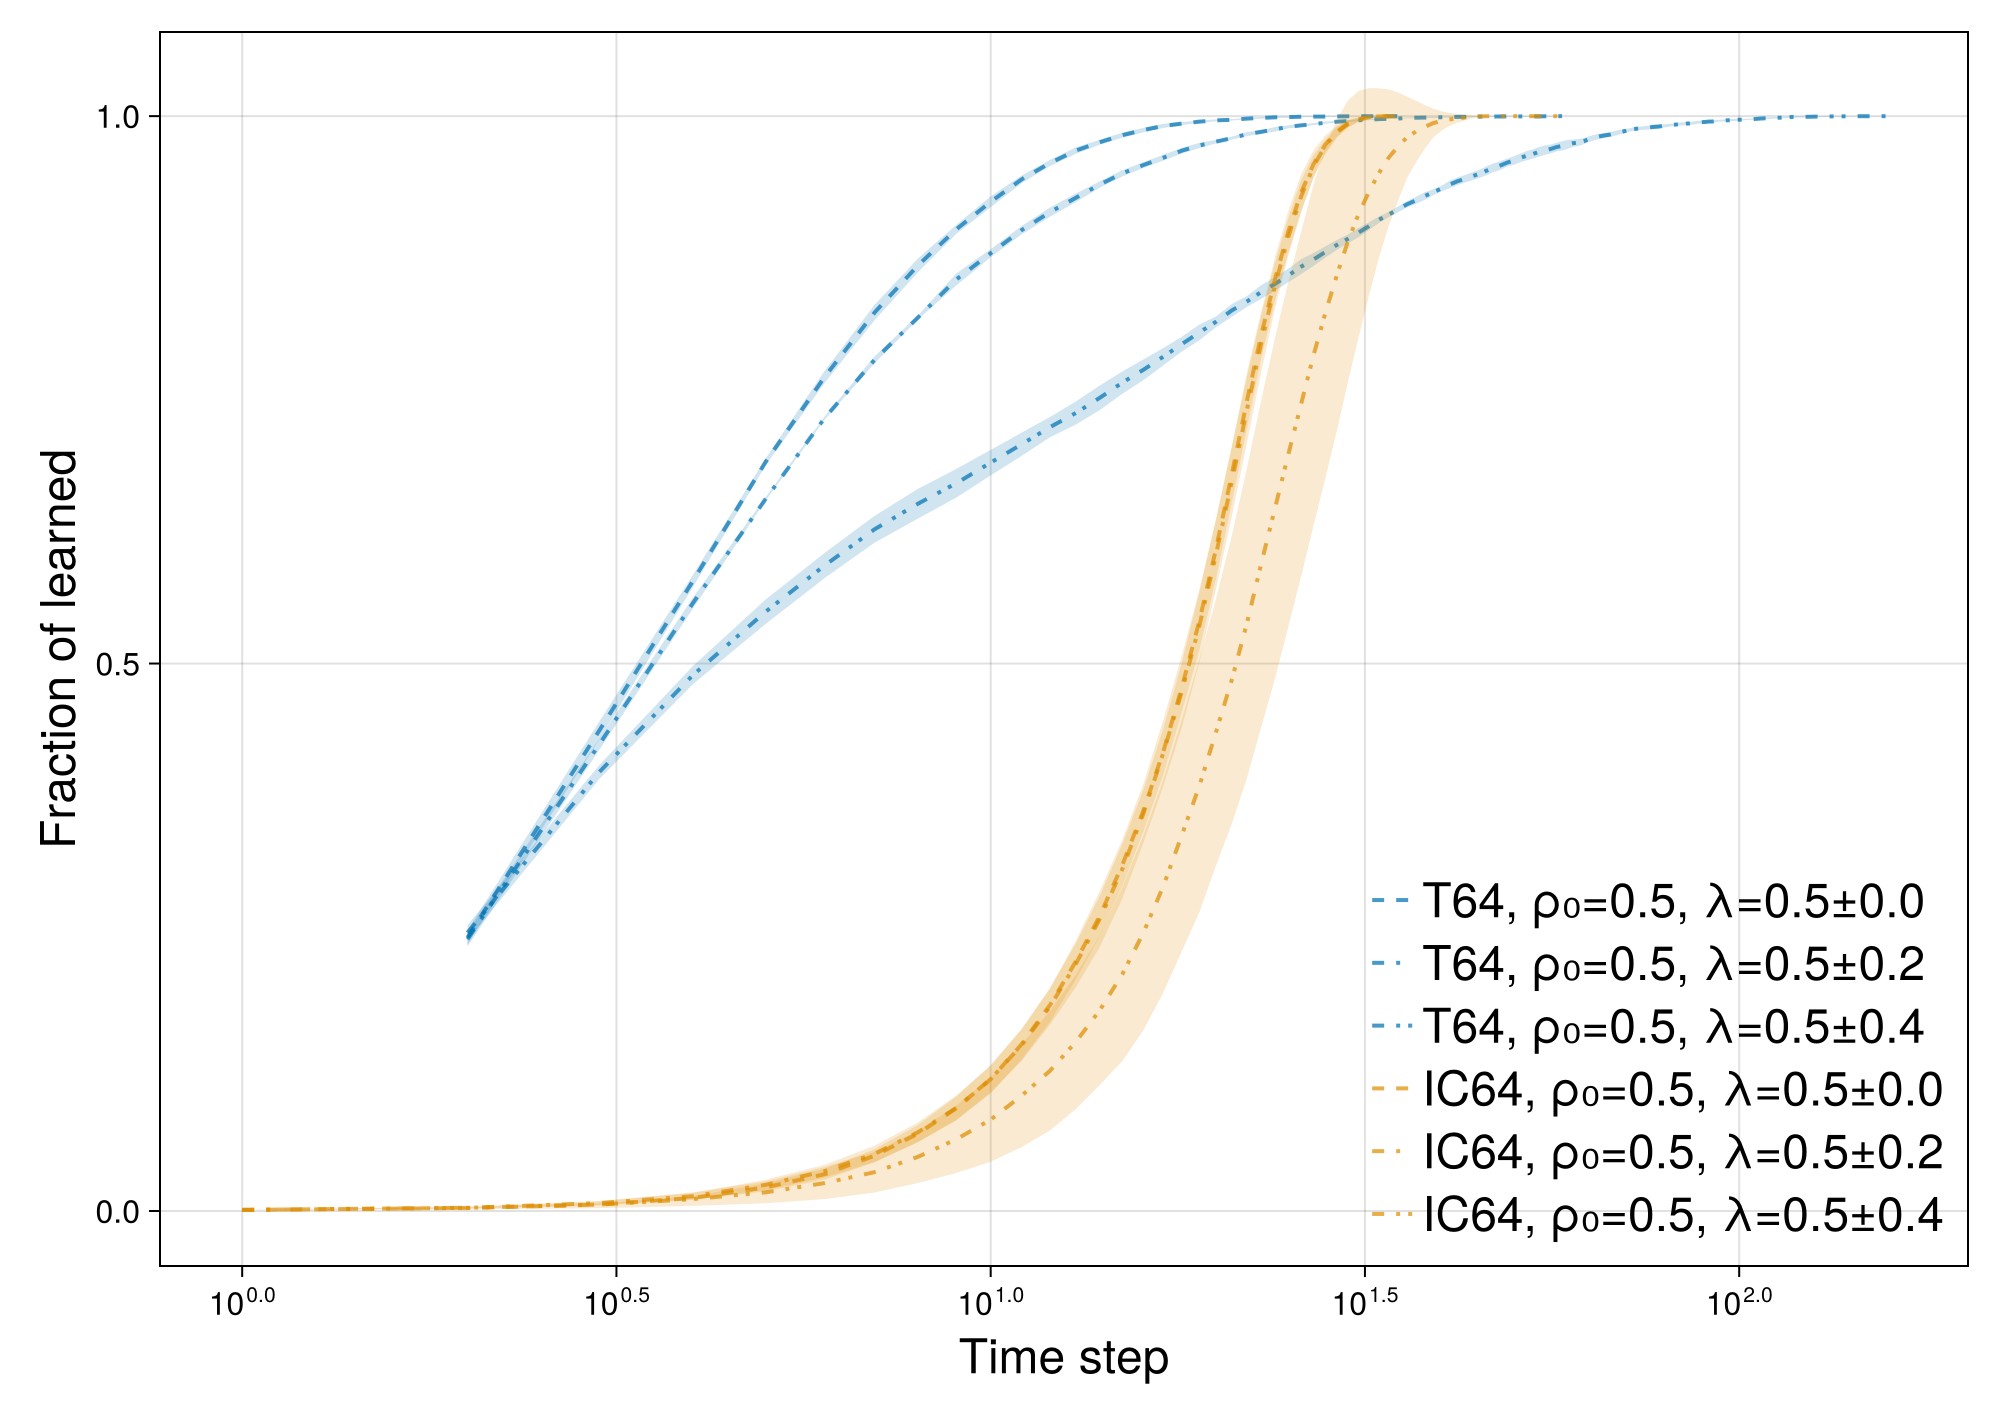
\includegraphics[width=0.45\textwidth]{figures/2D-BPCAIH-analysis/comparison plots/δλ.png}
            \caption{Comparison of time to learn $t_{\rm max}$ and fraction of learned students for different learning rate heterogeneity $\delta\lambda$.
            Each method of instruction corresponds to a different color --- blue for traditional, orange for inner corner.
            Different $\delta\lambda$ values correspond to different line styles where $\delta\lambda=0,0.2,0.4$ are represented by dashed lines, alternating dots and dashes, and two dots and a dash respectively.
            Other parameters are fixed at $N=64$ and $\rho_0=0.5$.
            The bands around each line show the standard deviation of the data over $20$ trials.
            Higher fraction of learned students indicate better learning.}
            \label{fig:comparison δλ}
        \end{figure}

        % We also investigate the effects of seating arrangement for PI in Figure~\ref{fig:comparison SA}.
        % For the set of parameters $L=64,\space\rho_0=0.5,\space\delta\lambda=0.2$, we find that the inner corner seating arrangement performs the best in terms of both the time it takes for all the students to learn and the classroom's learning rate.
        % Furthermore, we see that TI performs better than PI, especially for the earlier time steps.

        
        
        % Investigating this phenomenon further, we find that the learning curve for TI has two stages: a fast initial stage and a slow final stage.
        % The fast initial stage is characterized by a sharp increase in the number of learned students, this is caused by the majority of fast students learning quickly.
        % The slow stage is characterized by a much slower increase in the number of learned students, this is caused by waiting for the slower students to learn.
        % This phenomenon is seen in Figure~\ref{fig:comparison δλ} where the TI case where the students have a homogenous learning rate ($\delta\lambda=0$) show a consistent slope throughout the simulation compared to cases with heterogeneity ($\delta\lambda>0$) where the two-stage learning process is more evident.

        
        % This hypothesis is further supported when investigating specific cases where the two-stage learning process is expected to be more pronounced --- classes under TI with low positional learning factor $\rho_0$ and high learning rate heterogeneity $\delta\lambda$.
        % Figure~\ref{fig:two stage learning} shows one trial of a class under TI with $L=64$, $\rho_0=0.3$, and $\delta\lambda=0.4$.
        % We see that for $t=2$, the majority of the student that learned are those with higher learning rates ($\lambda=0.5+0.4$).
        % By $t=13$, the slower students have started to learn, but the rate of learning has slowed down significantly as the majority of students with higher learning rate have already learned.
        % This simulation will spend up to $t=232$ waiting for the slower students to learn.
        
    \begin{figure}[htbp!]
        \centering
        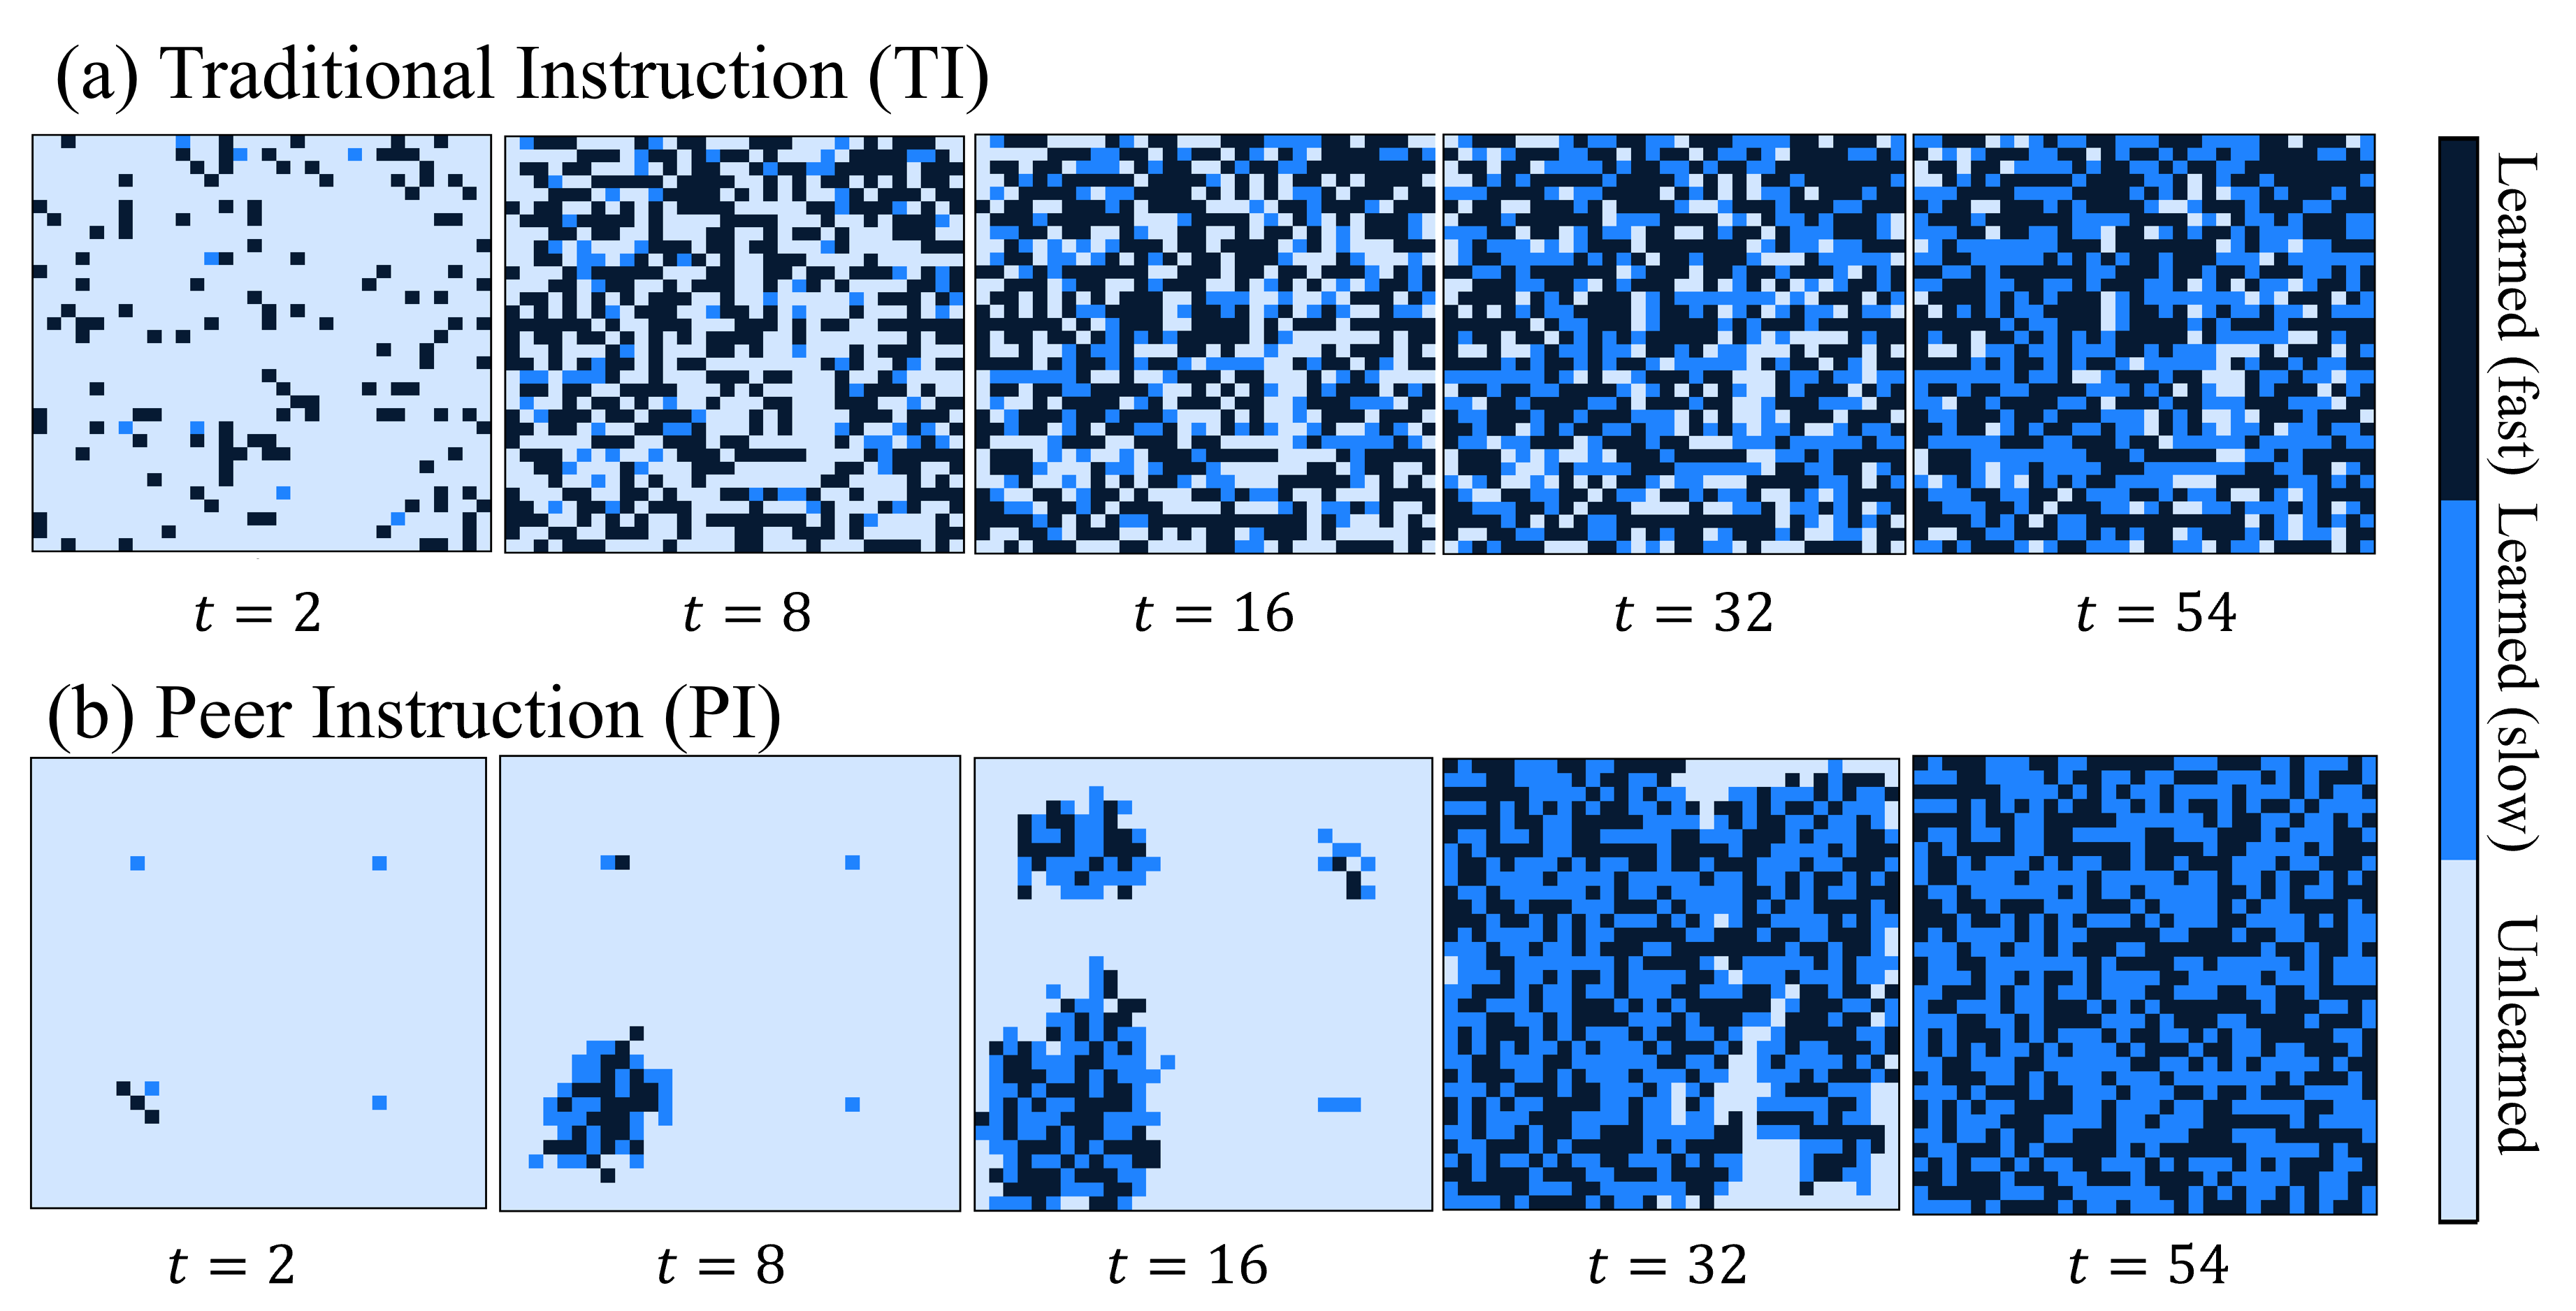
\includegraphics[width=0.45\textwidth]{figures/2D-BPCAIH-analysis/class evolutions/class_evolution.png}
        \caption{
            Example classroom evolution for with $L=32$, $\rho_0=0.3$, and $\delta\lambda=0.4$ at different time steps $t=2,8,16,32,54$.
            Dark blue cells represent learned students with learning rate $\lambda=\lambda_0+\delta\lambda$, blue cells represent learned students with learning rate $\lambda=\lambda_0-\delta\lambda$, and light blue cells represent unlearned students.
        }\label{fig:class_evolution}
    \end{figure}

    As for PI, varying the different parameters do not lead to as varied dynamics as TI.
    The progression of the fraction of learned students are affected the same way when varying class size $N$, positional learning factor $\rho_0$, and learning rate heterogeneity $\delta\lambda$.
    Generally, there is a time delay before the learning starts to speed up.
    As shown in Figure~\ref{fig:comparison size}, Figure~\ref{fig:comparison ρ₀}, and Figure~\ref{fig:comparison δλ}, increasing class size $N$ and learning rate heterogeneity $\delta\lambda$, and decreasing positional learning factor $\rho_0$ all increase this time delay.
    A combination of these factors may affect to the rate of classes' progression over time once learning speeds up, but these factors individually do not noticeably affect the progression.
    Additionally, we see in Figure~\ref{fig:comparison SA} that different SAs perform differently even with the same set of parameters with the inner corner SA performed the best.
    The random SA may outperform the center and outer corner SAs in the middle of the simulation but still ends up having the highest time to learn $t_{\rm max}$.


    \begin{figure}[htbp!]
        \centering
        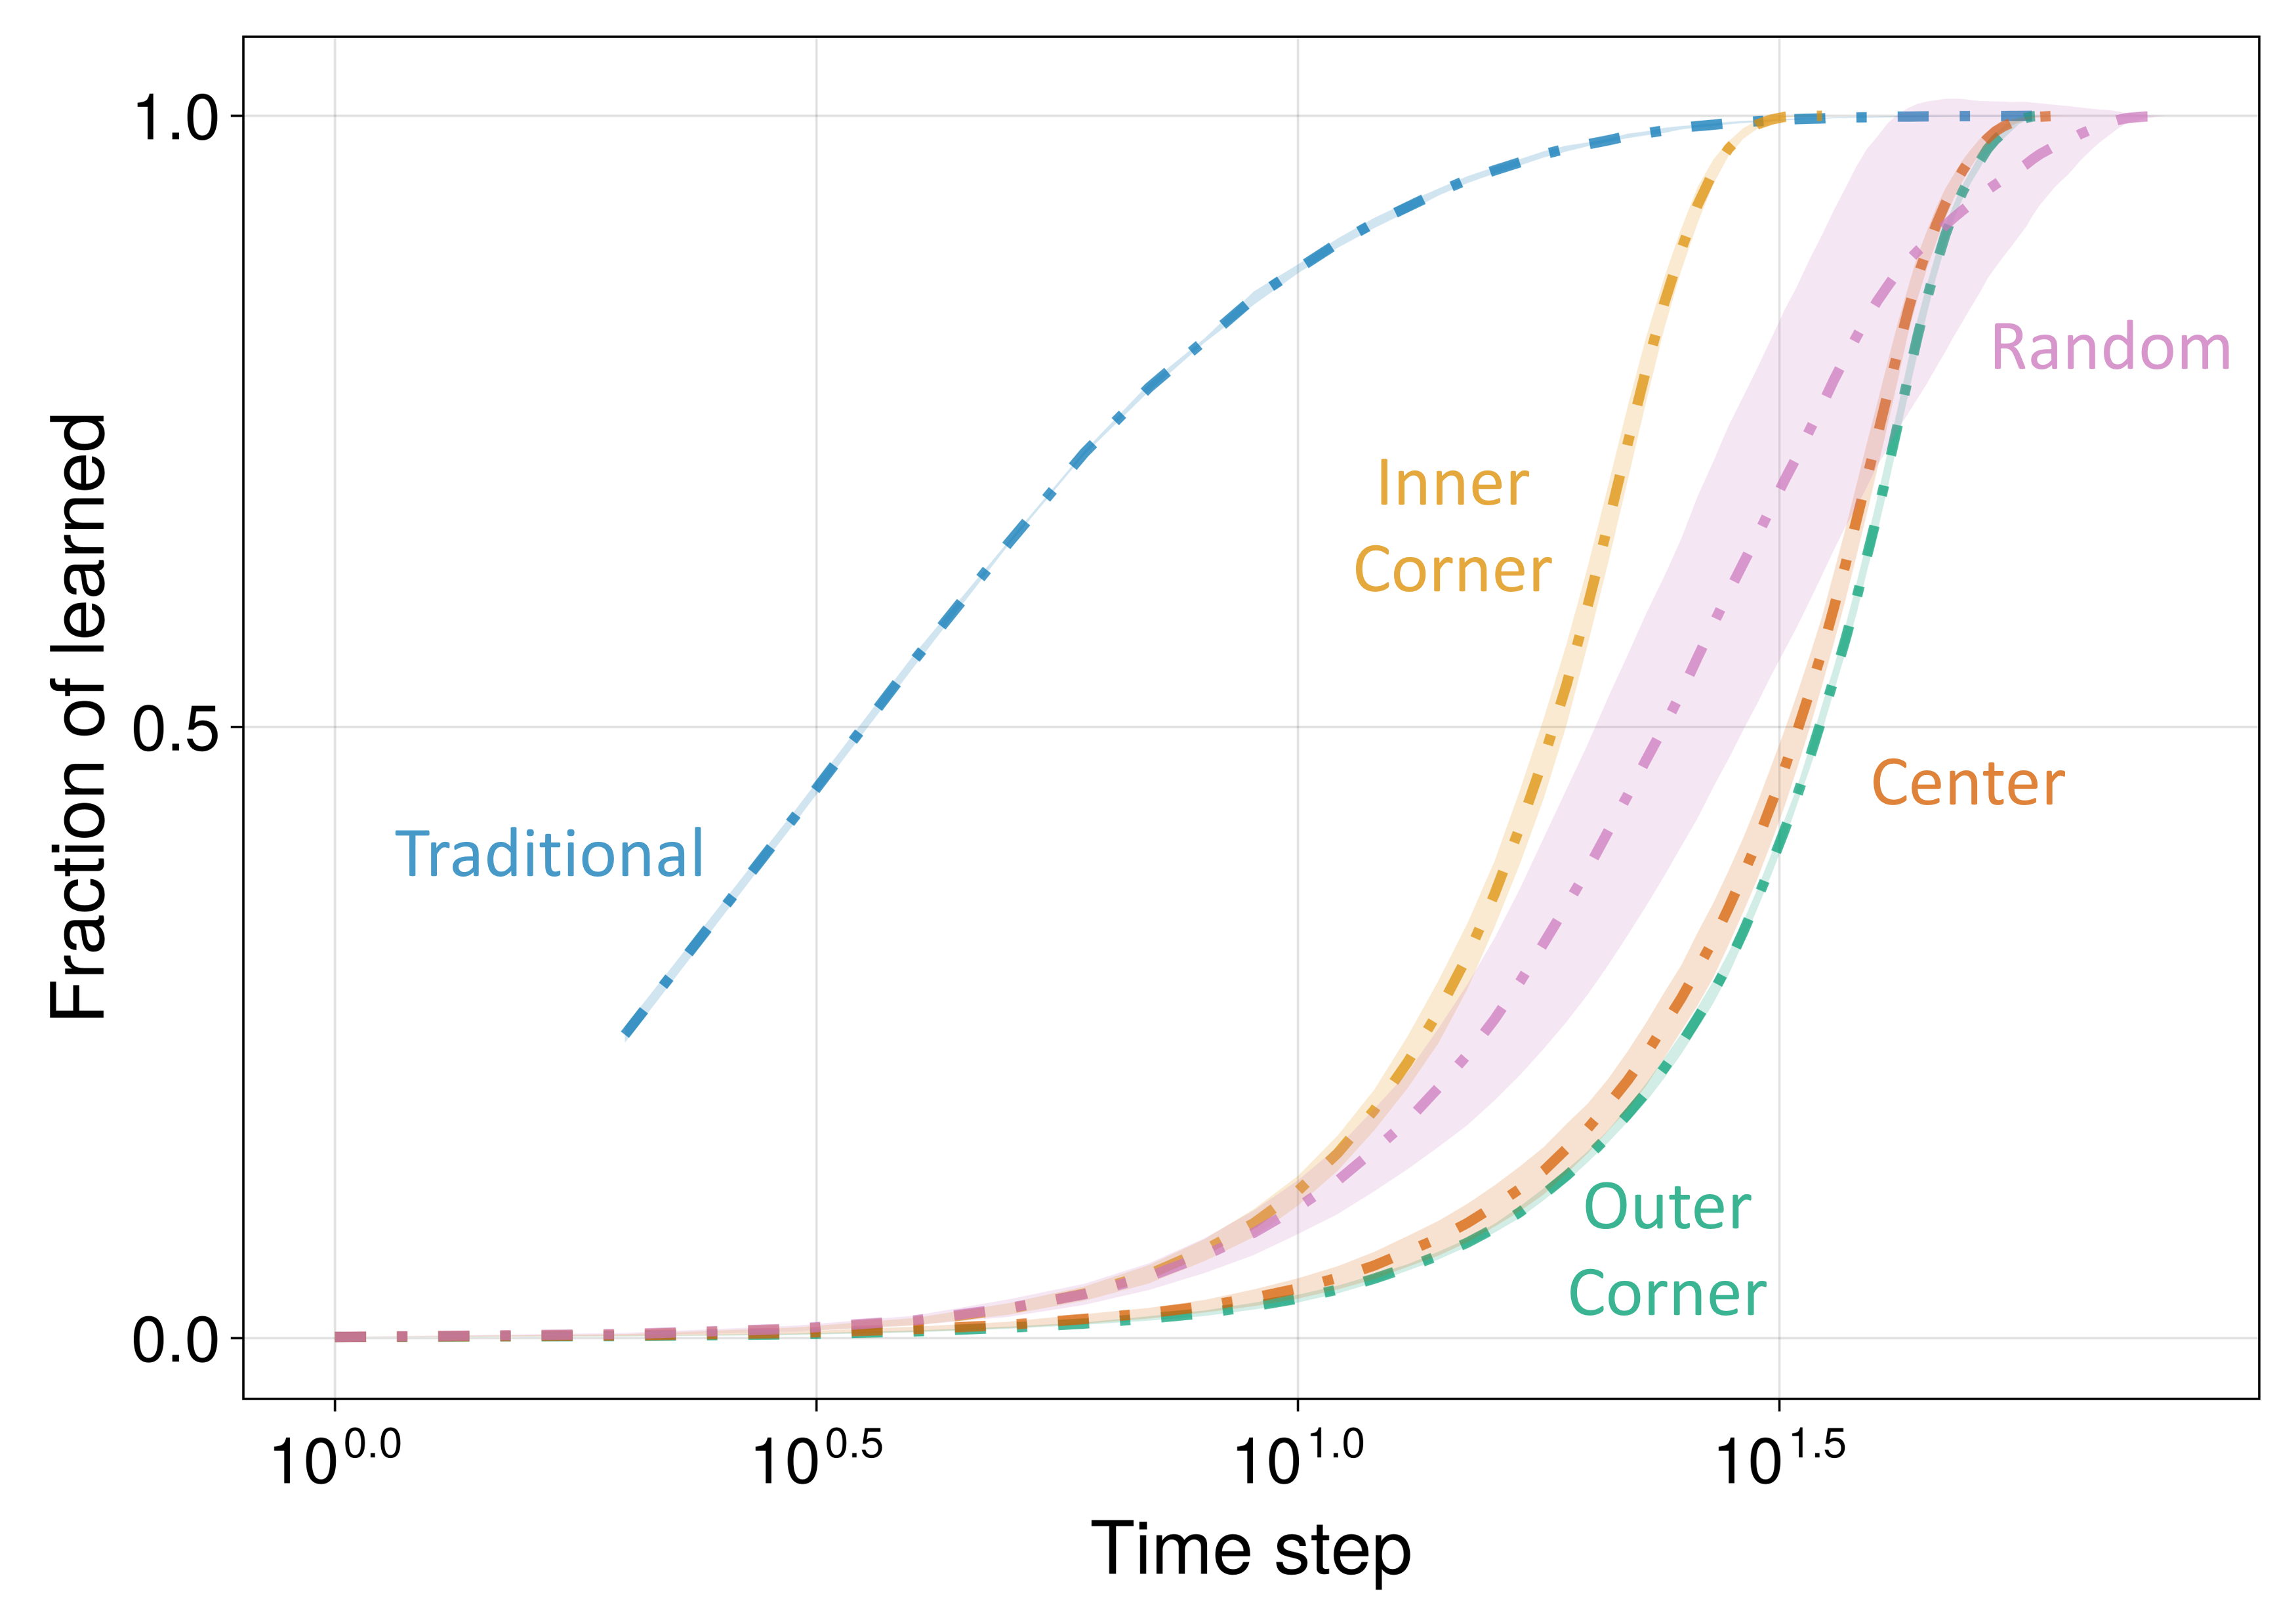
\includegraphics[width=0.45\textwidth]{figures/2D-BPCAIH-analysis/comparison plots/SA.png}
        \caption{Comparison of time to learn $t_{\rm max}$ and fraction of learned students for different SAs.
        Each SA corresponds to a different color --- blue for traditional, orange for inner corner, green for outer corner, orange for center, and pink for random.
        The bands around each line show the standard deviation of the data over 20 trials.
        Higher fraction of learned students indicate better learning.}
        \label{fig:comparison SA}
    \end{figure}

    The plots in this section show that classes under TI have more students learning in the earlier time steps, but has lower time to learn $t_{\rm max}$ when compared to classes under PI with the same set of parameters.
    However, we found that for cases of extremely high heterogeneity $\delta\lambda$ and low positional learning factor $\rho_0$, some simulations of TI did not finish with all students learned while PI did.
    For these cases, the time for all students to learn might be longer than the $t_{\rm max}$ value we obtained.
    Nevertheless, these findings suggest that to optimize the learning in the classroom, it would be best to perform TI at the start of the class to take advantage of the fast initial learning stage, then switch to PI where having learned students spread throughout the classroom benefit those who have yet to learn.
    This is consistent with current practices~\cite{mazur1997peer,smith2009peer,lasry2008peer,roxas2010seating}, where the students are expected to have read up on the material in advance and the instructor gives a short lecture before the students engage in peer discussion.

    \subsection{Summary of effects of class size $N$, positional learning factor $\rho_0$, and learning rate heterogeneity $\delta\lambda$}
        
        As we vary the different parameters, as shown in Figure~\ref{fig:Params effect summary t}, we are able to identify which cases are more favorable for TI or PI.
        We find that PI suffers more than TI when handling larger class sizes $N$, and that TI suffers more from increased learning rate heterogeneity $\delta\lambda$ compared to PI.
        However, low positional learning factor $\rho_0$ affects both TI and PI similarly.

        The same figure also shows us the magnitude of the advantage of one method of instruction over the other.
        We find that when TI is advantageous, like in cases of big classrooms and low learning rate heterogeneity, the advantage over PI is not that large.
        However, in cases where PI is advantageous, like in cases of small classrooms and high learning rate heterogeneity, the advantage over TI is very large.
        This suggests that PI can be a safe option --- never performing much worse than TI, but can perform much better in certain cases.

        \begin{figure}[htbp!]
            \centering
            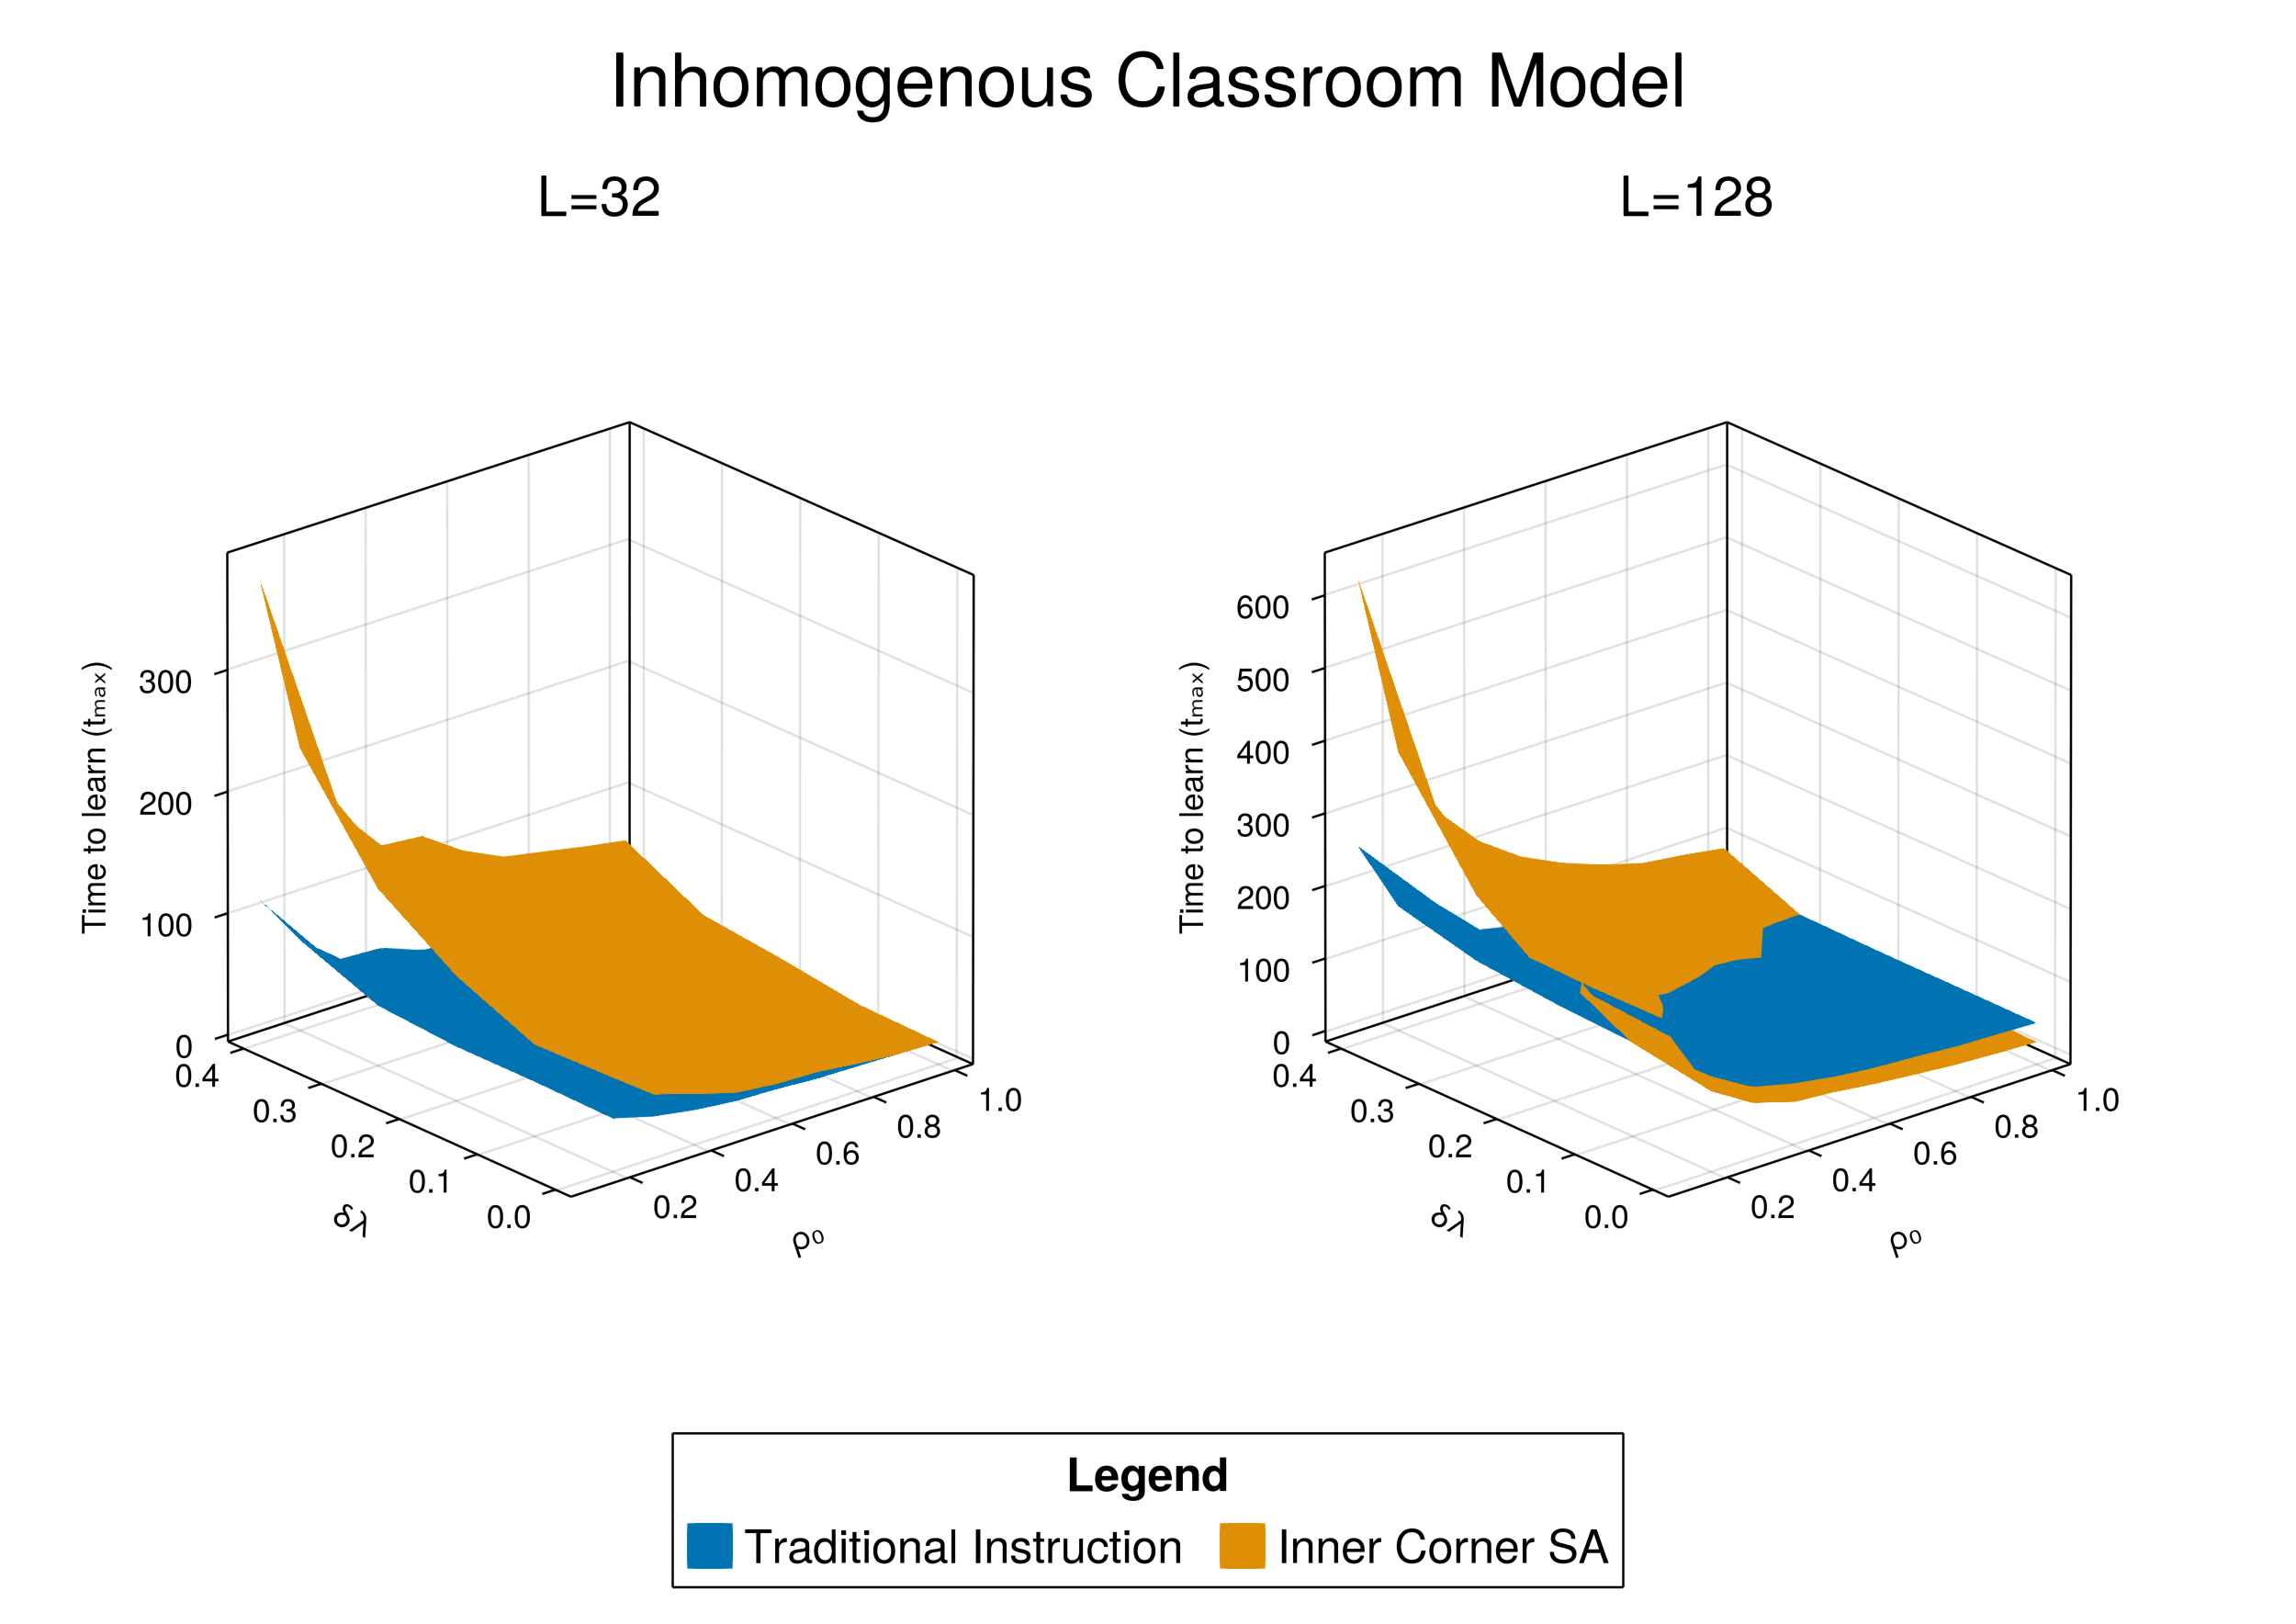
\includegraphics[width=0.47\textwidth]{figures/2D-BPCAIH-analysis/rho-dl-t plots/32-128 comparison.png}
            \caption{Time to learn $t_{\rm max}$ as a function of positional learning factor $\rho_0$ and heterogeneity $\delta\lambda$ of PI (inner corner SA) and TI for different class sizes $N=L^2$.
            The blue surface represent TI and the orange surface represents PI.
            Lower time to learn indicates better learning.}
            \label{fig:Params effect summary t}
        \end{figure}

    \subsection{Existing research data}
        
        Comparing our data to Nitta's model (Equation~\ref{eq:nitta_model})~\cite{nitta2019mathematical}, as in Figure~\ref{fig:Return map}, only our data for PI approaches their model --- this is expected since their model is for PI and not TI.
        Furthermore, PI only approaches their model when the conditions are favorable for PI (Figure~\ref{fig:return_map_fav}).
        Considering that their model has been shown to agree with experimental data, it suggests that real world students' behavior and learning dynamics are better represented by the values of high positional learning factor $\rho_0$ and small class sizes $N$.
        It should also be noted that Nitta's model and data tracks individual students' learning while our model tracks the class's learning as a whole.
        We chose to track learning this way because there is not much insight to be gained from tracking individual students' learning in a binary-state model.
        Hence, we used the fraction of learned students $f_t$ in place of Nitta's usage of students' test scores for $S_t$.
        Nevertheless, the agreement of our model to theirs and to experimental data suggests that our model can be a good approximation of the real world with further improvements.

        \begin{figure}[htbp!]
            \centering
            \subfigure[$L=128,\space\rho_0=0.1,\space\lambda=0.5\pm0.4$]{\label{fig:return_map_unfav}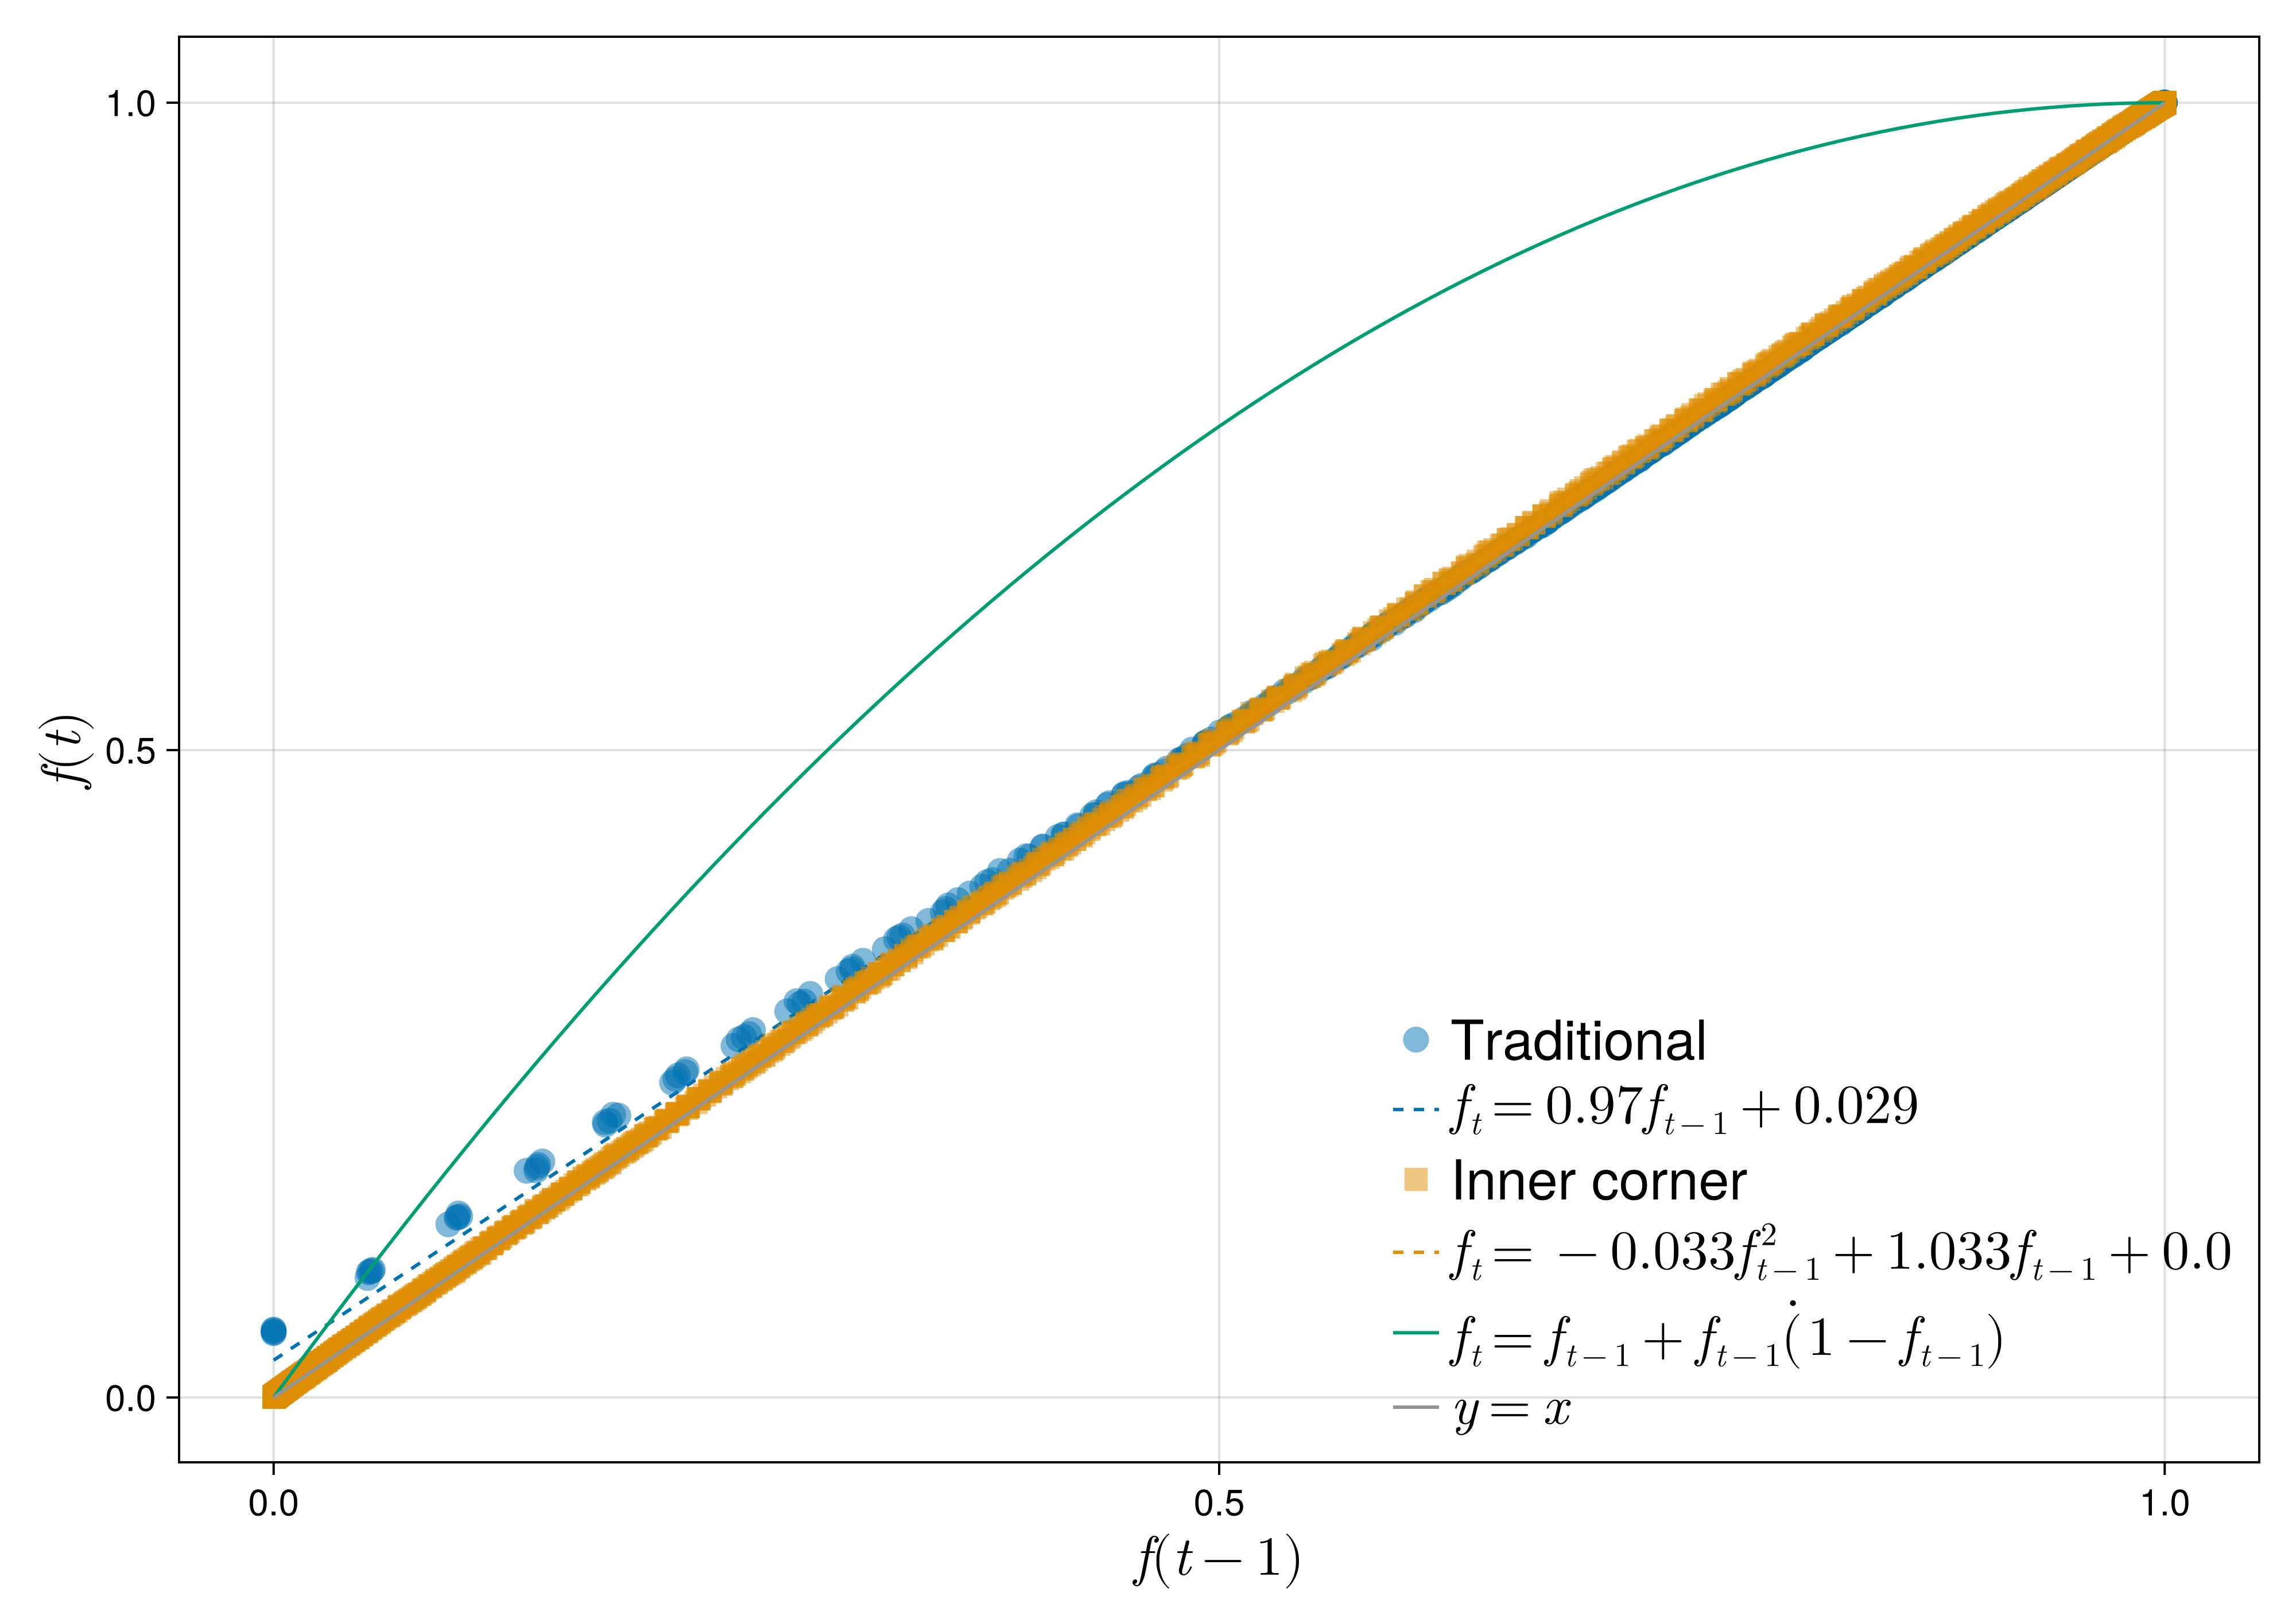
\includegraphics[width=0.47\textwidth]{figures/2D-BPCAIH-analysis/return plots/return-map-128-0.1-0.5-0.4.png}}
            \subfigure[$L=32,\space\rho_0=0.9,\space\lambda=0.5\pm0.0$]{\label{fig:return_map_fav}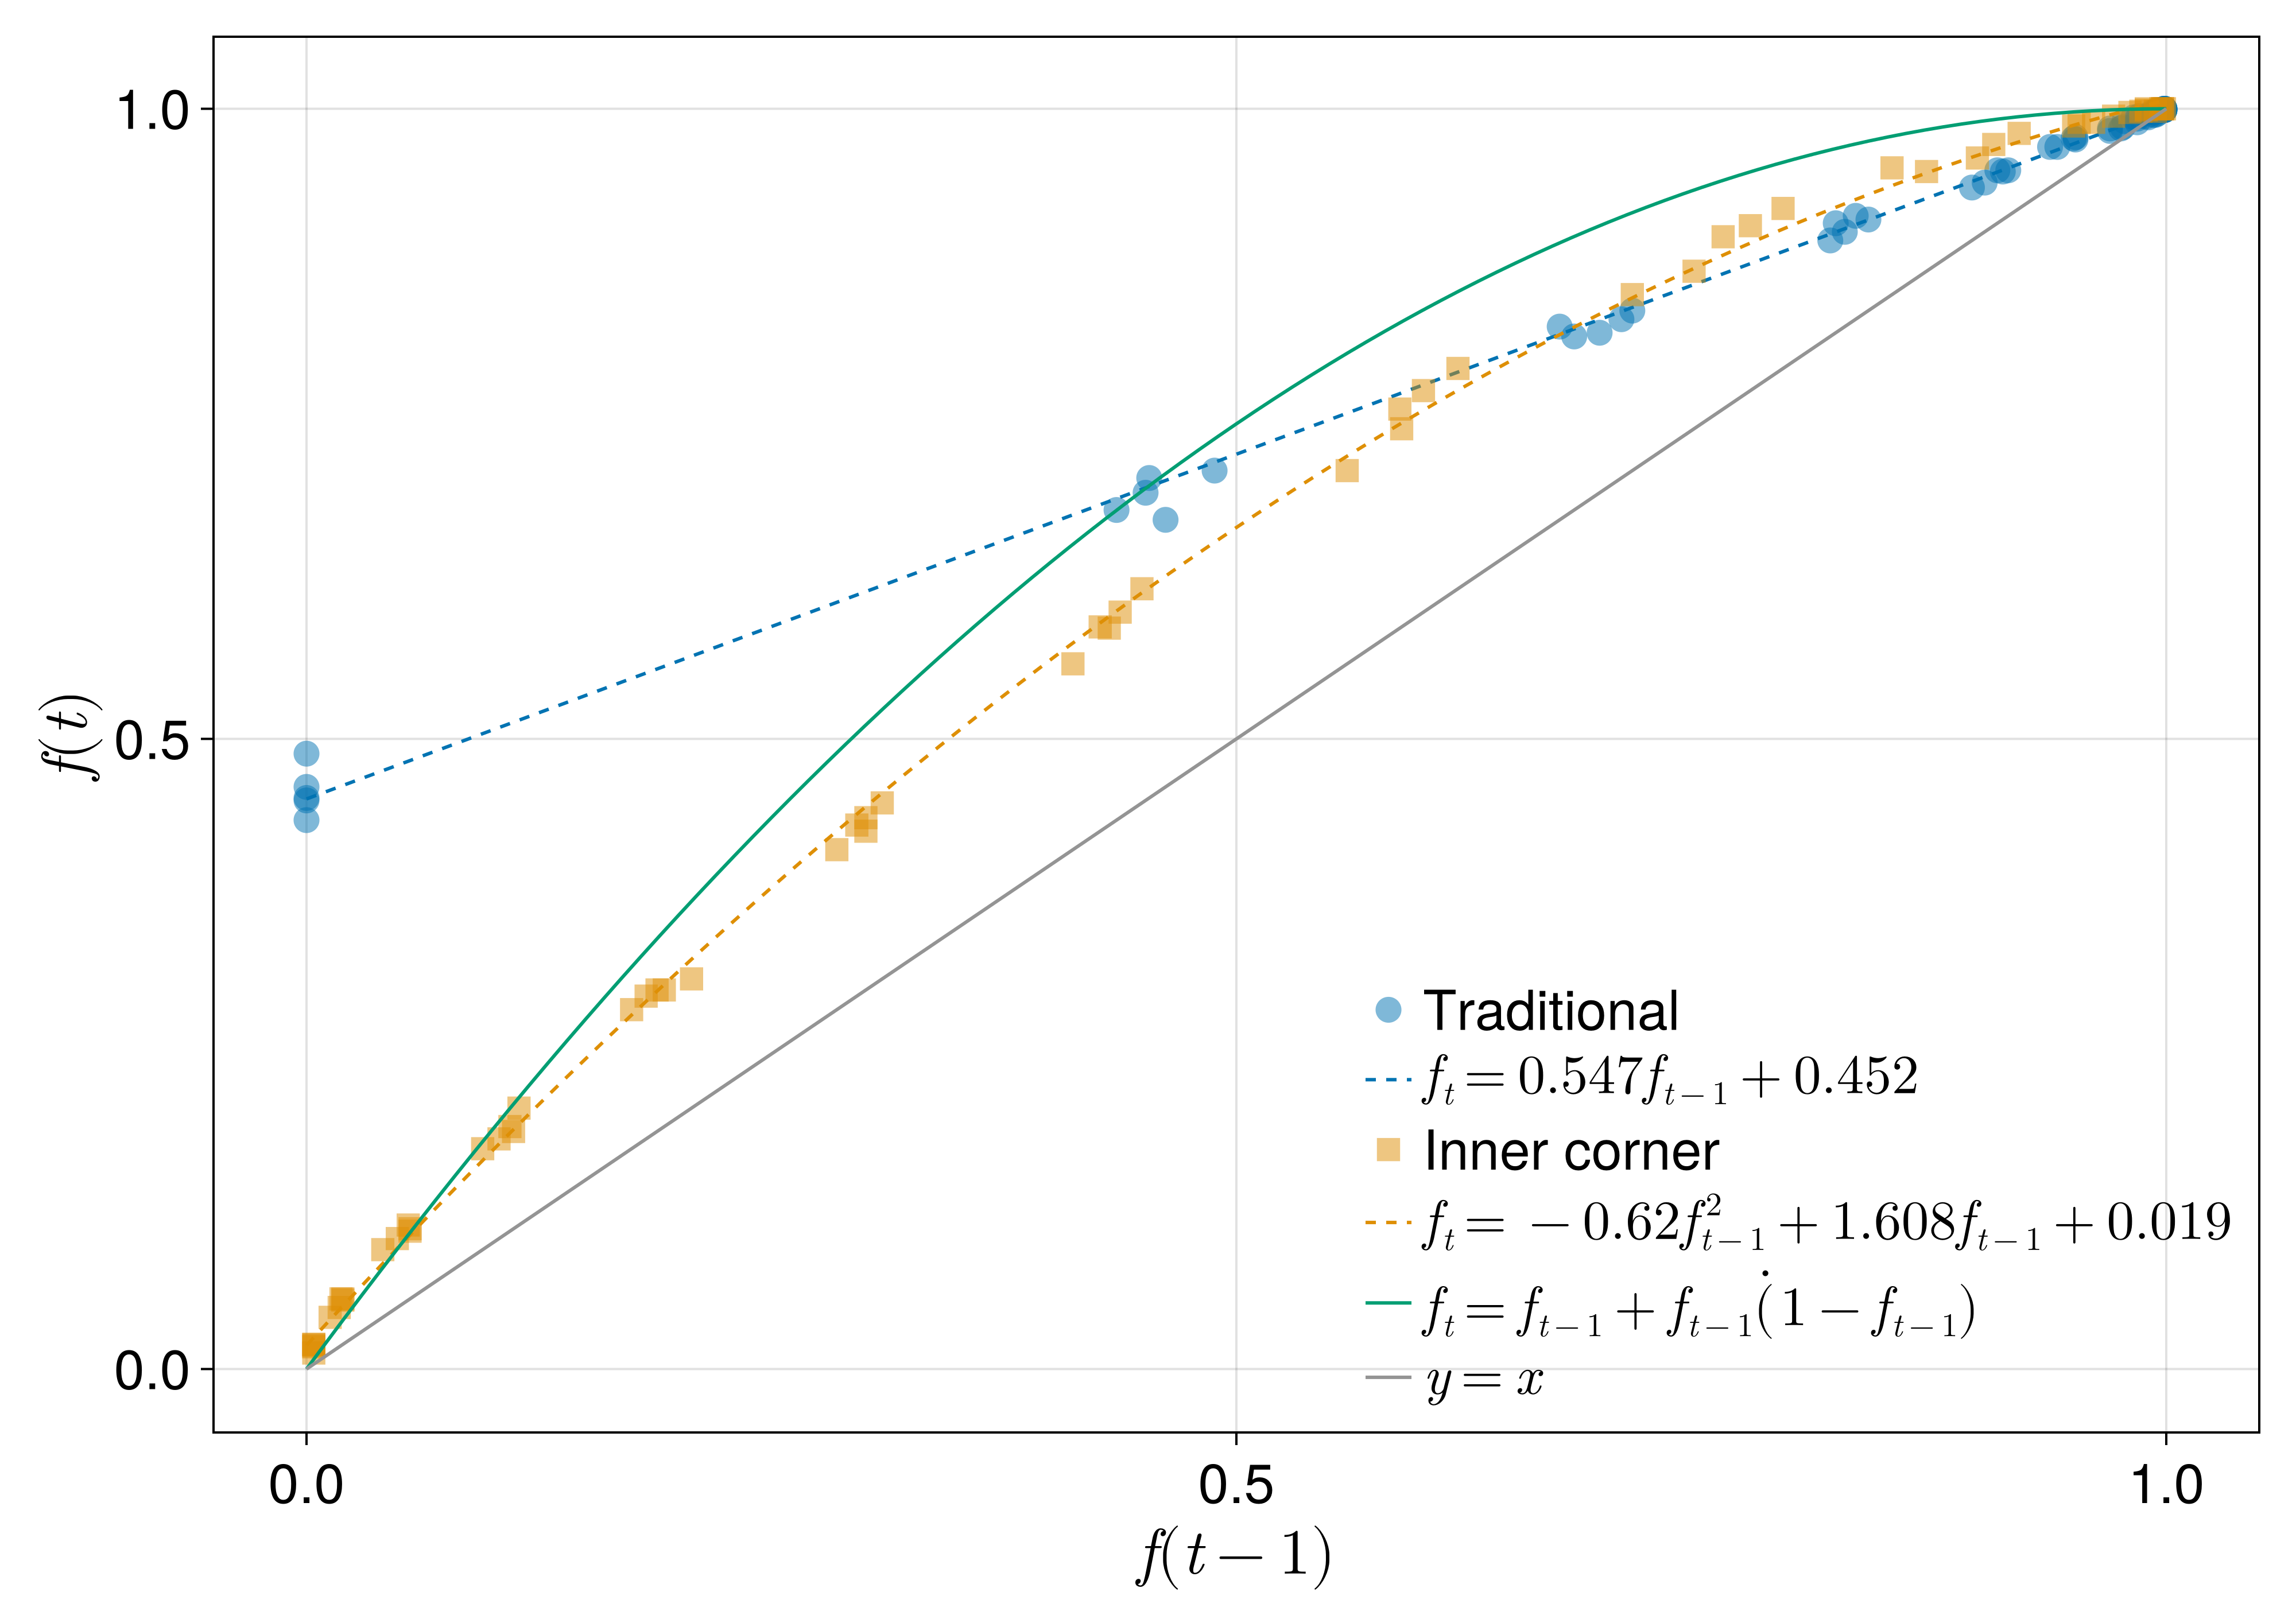
\includegraphics[width=0.47\textwidth]{figures/2D-BPCAIH-analysis/return plots/return-map-32-0.9-0.5-0.0.png}}
            \caption{Return map for selected parameter sets for both TI and PI.
            Blue circles represent the data points for TI and orange squares represent the data points for PI.
            The corresponding best-fit quadratic function obtained using the Levenberg-Marquardt algorithm for each set of data points are shown in blue and orange dashed lines respectively.
            The green line represents Nitta's theoretical model (Equation~\ref{eq:nitta_model}) and the gray line represents $y=x$.}
            \label{fig:Return map}
        \end{figure}

        Following Nitta's model and equation for gain (Equation~\ref{eq:nitta_model} and \ref{eq:nitta_gain}), we can see for our PI model where
%
        \begin{equation}
            \label{eq:PI_ft_eq}
            f_{t+1} \approx a + bf_t + cf_t^2
        \end{equation}
%
        $b$ is expected to be $b=1-c$ and the gain $g$ is
%
        \begin{equation}
            \label{eq:PI_g_eq}
            g \approx a + cf_t
        \end{equation}

        Doing the same for our TI model which was best modeled by a linear function
%
        \begin{equation}
            \label{eq:TI_ft_eq}
            f_{t+1} \approx f_t + g(1-f_t) \approx m_0 + m_1f_t
        \end{equation}
%
        and noting that the coefficients $m_0$ and $m_1$ approximately sums to $1$ (Figure~\ref{fig:Return map}) gives us the equation for gain:
%
       \begin{equation}
            \label{eq:TI_g_eq}
            g \approx m_0
       \end{equation}

       These values for gain $g$ shows us that gains for TI are constant while gains for PI are linearly proportional to the fraction of learned students $f_t$.
       We find these values reasonable since TI is set up such that all students learn at the same time from the teacher while PI is set up such that students learn from each other.

        Compared to Roxas' work~\cite{roxas2010seating} which found the outer corner SA to perform the best, we found the inner corner SA to perform the best.
        This difference can be attributed to the simplifications made in our model.
        We were not able to consider the aptitude similarity effect that happens where students of similar aptitude learn better when grouped together regardless of their actual aptitude level~\cite{smith2009peer}.
        The implementation of this phenomenon is better suited for a continuous-state model rather than a binary-state model.
        Additionally, we did not consider the orientation of the students in the classroom, resulting in an isotropic system.
        In addition to the findings regarding seating arrangements, our model also agrees with their findings that homogenous classes find better improvements compared to heterogeneous classes.
    
\section{Summary and Conclusion}
    We propose a probabilistic cellular automata model as a new way of investigating learning dynamics in the classroom.
    Through this model, we can investigate how different factors can affect students' learning in the classroom for both traditional instruction (TI) and peer instruction (PI).

    We found that TI performs better in larger classes and when the students have low learning rate heterogeneity.
    On the other hand, PI performs better in smaller classes and when the students have high learning rate heterogeneity.
    To be more precise, class size, heterogeneity, and low positional learning factor affect both TI and PI negatively, but TI is not as affected by class size compared to PI and PI is not as affected by heterogeneity compared to TI.

    We also found that when a highly heterogeneous class is under TI, the class exhibits a two-stage learning process where majority of the fast students learn in the first few time steps and the rest of the time is spent waiting for slower students to learn. Our findings regarding class heterogeneity are in line with those of Roxas, et al. (2010)~\cite{roxas2010seating}.
    However, our findings regarding seating arrangement differ from theirs where they found that the outer corner seating arrangement perform best while we found that the inner corner seating arrangement perform best.
    This difference is likely because of the simplifications made in our model --- namely learning isotropy and non-implementation of an aptitude similarity effect.
    These simplifications are from the limitations of having a binary-state model.

    Another limitation of having a binary-state model is that there are not much insight to be gained from tracking individual students' learning.
    Hence, we chose to track the class's learning as a whole.
    Despite having a different way to assess the methods of instruction effectiveness, our findings are consistent with the existing works like that of Nitta, et al.~\cite{nitta2019mathematical} which is backed by real-world data.

    While our model can be a good approximation of the real world, there are still improvements that can be made.
    The current model only considers the peer discussion part of a whole PI session.
    A mixed model that considers the whole session with a mix of TI and TI would be a better representation of the real world.
    Additionally, transitioning to a continuous-state model would allow us to incorporate more real-world phenomena like aptitude similarity and orientation effects.


\bibliography{biblio}

\end{document}

